\documentclass[8pt]{beamer}

%%pacotes referentes ao Beamer
%\useoutertheme{split}
%\setbeamertemplate{navigation symbols}{}

%\usetheme{beamertheme}
%\usebeamercolor{beamer-color name}

%\usetheme{Boadilla}
%\usecolortheme{dove}

\usetheme{Montpellier}
\usecolortheme{beaver}

% \usetheme{pittsburgh}
% \usecolortheme{dolphin}
%\usecolortheme{dove}
%\usecolortheme{seahorse}

%\usetheme{Montpellier}

%number in figures an tables -- beamer
\setbeamertemplate{caption}[numbered]

%Colocar no description
%[leftmargin=!,labelwidth=\widthof{Turma A}]
	
%pacotes usuais do latex
\usepackage[portuguese]{babel}
\usepackage[utf8]{inputenc}
\usepackage{bm}
\usepackage{graphicx}
\usepackage{subfig}
\usepackage[round]{natbib}
\usepackage{tikz}
\usetikzlibrary{shapes,arrows}
\usepackage{natbib}
\usepackage{times}
\usepackage{calc} %computes the length of a string
\usepackage{dsfont} %pacote para o 1 estilisado para indicadora
\usepackage{enumerate} %permite fazer uns enumerates diferentes
\usepackage[font=small,labelfont=bf]{caption} %permite colocar um segundo caption
\usepackage{booktabs} % comando \toprule, \midrule e \bottomrule
\usepackage{times} %times new roman font
\usepackage{multirow} %comando \multirow
\usepackage{setspace}
\usepackage{xcolor} %texto colorido
\usepackage{booktabs} %costumized tabs
\usepackage{physics} %absolute value
\usepackage{xcolor}
\usepackage{bigints}

% setting color
\definecolor{important}{RGB}{0,153,0}

%código para alinhar a esquerda os itens no description
\defbeamertemplate{description item}{align left}{\insertdescriptionitem\hfill}
\defbeamertemplate{enumerate item}{align left}{\insertdescriptionitem\hfill}



%AMS packages
\usepackage{amsmath}
\usepackage{amsfonts}
\usepackage{amssymb}

%Não quebre linhas
\binoppenalty=\maxdimen
\relpenalty=\maxdimen

%Comandos criados por mim
\DeclareMathOperator*{\argmin}{arg\,min}

\DeclareMathOperator*{\argmax}{arg\,max}


\DeclareMathOperator{\espe}{E}

\DeclareMathOperator{\spann}{span}

\DeclareMathOperator{\cov}{Cov}

\DeclareMathOperator{\vari}{Var}

\DeclareMathOperator{\positivo}{positivo}

%Informações para o primeiro slide
\date{}
\title[Regressão linear]{Regressão linear simples}
\author[Gilberto Sassi]{Gilberto Pereira Sassi}
\institute[IME -- UFBA]{Universidade Federal da Bahia \\ Instituto de Matem\'{a}tica e Estat\'{i}stica\\ Departamento de Estat\'{i}stica }

\begin{document}
	
\tikzstyle{decision} = [diamond, draw, fill=blue!20, 
text width=4.5em, text badly centered, node distance=3cm, inner sep=0pt]
\tikzstyle{block} = [rectangle, draw, fill=blue!20, 
text width=5em, text centered, rounded corners, minimum height=4em]
\tikzstyle{line} = [draw, -latex]
\tikzstyle{cloud} = [draw, ellipse,fill=red!20, node distance=3cm,
minimum height=2em]
	
\begin{frame}{}
	\maketitle
\end{frame}

\section{Regressão linear simples}

\begin{frame}{Motivação: Regressão linear simples}

\begin{block}{Modelo determinístico}
	\textcolor{important}{Modelo matemático não inclui incerteza ou aleatoriedade.} Por exemplo, considere a posição inicial $d_0$ de corpo e a velocidade $v$, então a posição deste corpo no momento $t$ é dado por
	$$d_t = d_0 + v \cdot t.$$
\end{block}
\vfill

\begin{block}{Modelo estatístico}
	\textcolor{important}{Modelo matemático inclui incerteza ou aleatoriedade.} Por exemplo, considere $y$ o consumo de energia elétrica de uma residência  e $x$ o tamanho em metros quadrados da casa. Casas maiores tendem a gastar mais energia elétrica, mas algumas podem ser econômicas e gastarem menos e outras podem gastar mais. Então, o consumo de energia elétrica pode ser descrita pelo modelo:
	$$y = a + b\cdot x + \epsilon.$$
	
	Uso pode ser inspirado através:
	\begin{itemize}
		\item Justificativa teórica;
		\item Diagrama de dispersão. Os pontos $(x_i, y_i)$ estão próximos da reta $y = a + b \cdot x$.
	\end{itemize}

	Assumimos que $\epsilon \sim N(0, \sigma^2)$.
\end{block}


\end{frame}

\begin{frame}{Regressão linear simples}

\footnotesize	
	\begin{block}{Apresentação: regressão linear simples}
		
		Sejam $X$ e $Y$ duas variáveis quantitativas associadas com valores observados conforme ilustrado na Tabela~\ref{tab:motivacao}.
		\begin{table}[htbp]
			\centering
			\caption{Observações de $X$ e $Y$.}
			\label{tab:motivacao}
			\begin{tabular}{l|ccc}
				\toprule[0.05cm]
					$X$ & $x_1$ & $\cdots$ &  $x_n$\\
					\midrule[0.05cm]
					$Y$ & $y_1$ & $\cdots$ &  $y_n$\\
				\bottomrule[0.05cm]
			\end{tabular}
		\end{table}
	
	Queremos encontrar valores $a$, chamado de intercepto, e $b$, chamado de inclinação, tal que 
	\begin{align*}
		y_i = a + b x_i + \epsilon_i, \quad i =1, \dots,n,
	\end{align*}
	e $a$ e $b$ é o valor que minimiza $S(a,b) = (y_1 - a - b x_1)^2+\dots + (y_n - a - b x_n)^2$.
	\end{block}

\begin{block}{Interpretação}
	Considere o método descrito pela equação $y = a + b \cdot x + \epsilon$.
	\begin{itemize}
		\item a parte $y = a + b \cdot x$ representa os valores de $y$ que podem ser  explicados por $x$ através da equação da reta $y = a + b \cdot x$;
		\item $\epsilon$ representa a parte dos valores de $y$ que não podem ser explicados por por $x$ através da equação da reta $y = a + b \cdot x$;
		\item chamamos $x$ de variável independente,  variável regressora ou variável explicativa;
		\item  chamamos de $y$ de variável dependente ou variável reposta.
	\end{itemize}
Os valores $\epsilon$ idealmente são pequenos, com média zero e com distribuição normal e com variância $\sigma^2$. A Figura~\ref{fig:motivacao} ilustra a ideia da regressão linear simples.
\end{block}
\normalsize

\end{frame}

\begin{frame}{Ilustração da regressão linear simples}
	
	Desejamos encontrar $a$ e $b$ de tal que forma que as distâncias $(y_i-a-bx_i)$ sejam as menores possíveis (em valores quadráticos).
	\begin{figure}[htbp]
		\centering
		\caption{Motivação de regressão linear simples.}
		\label{fig:motivacao}
		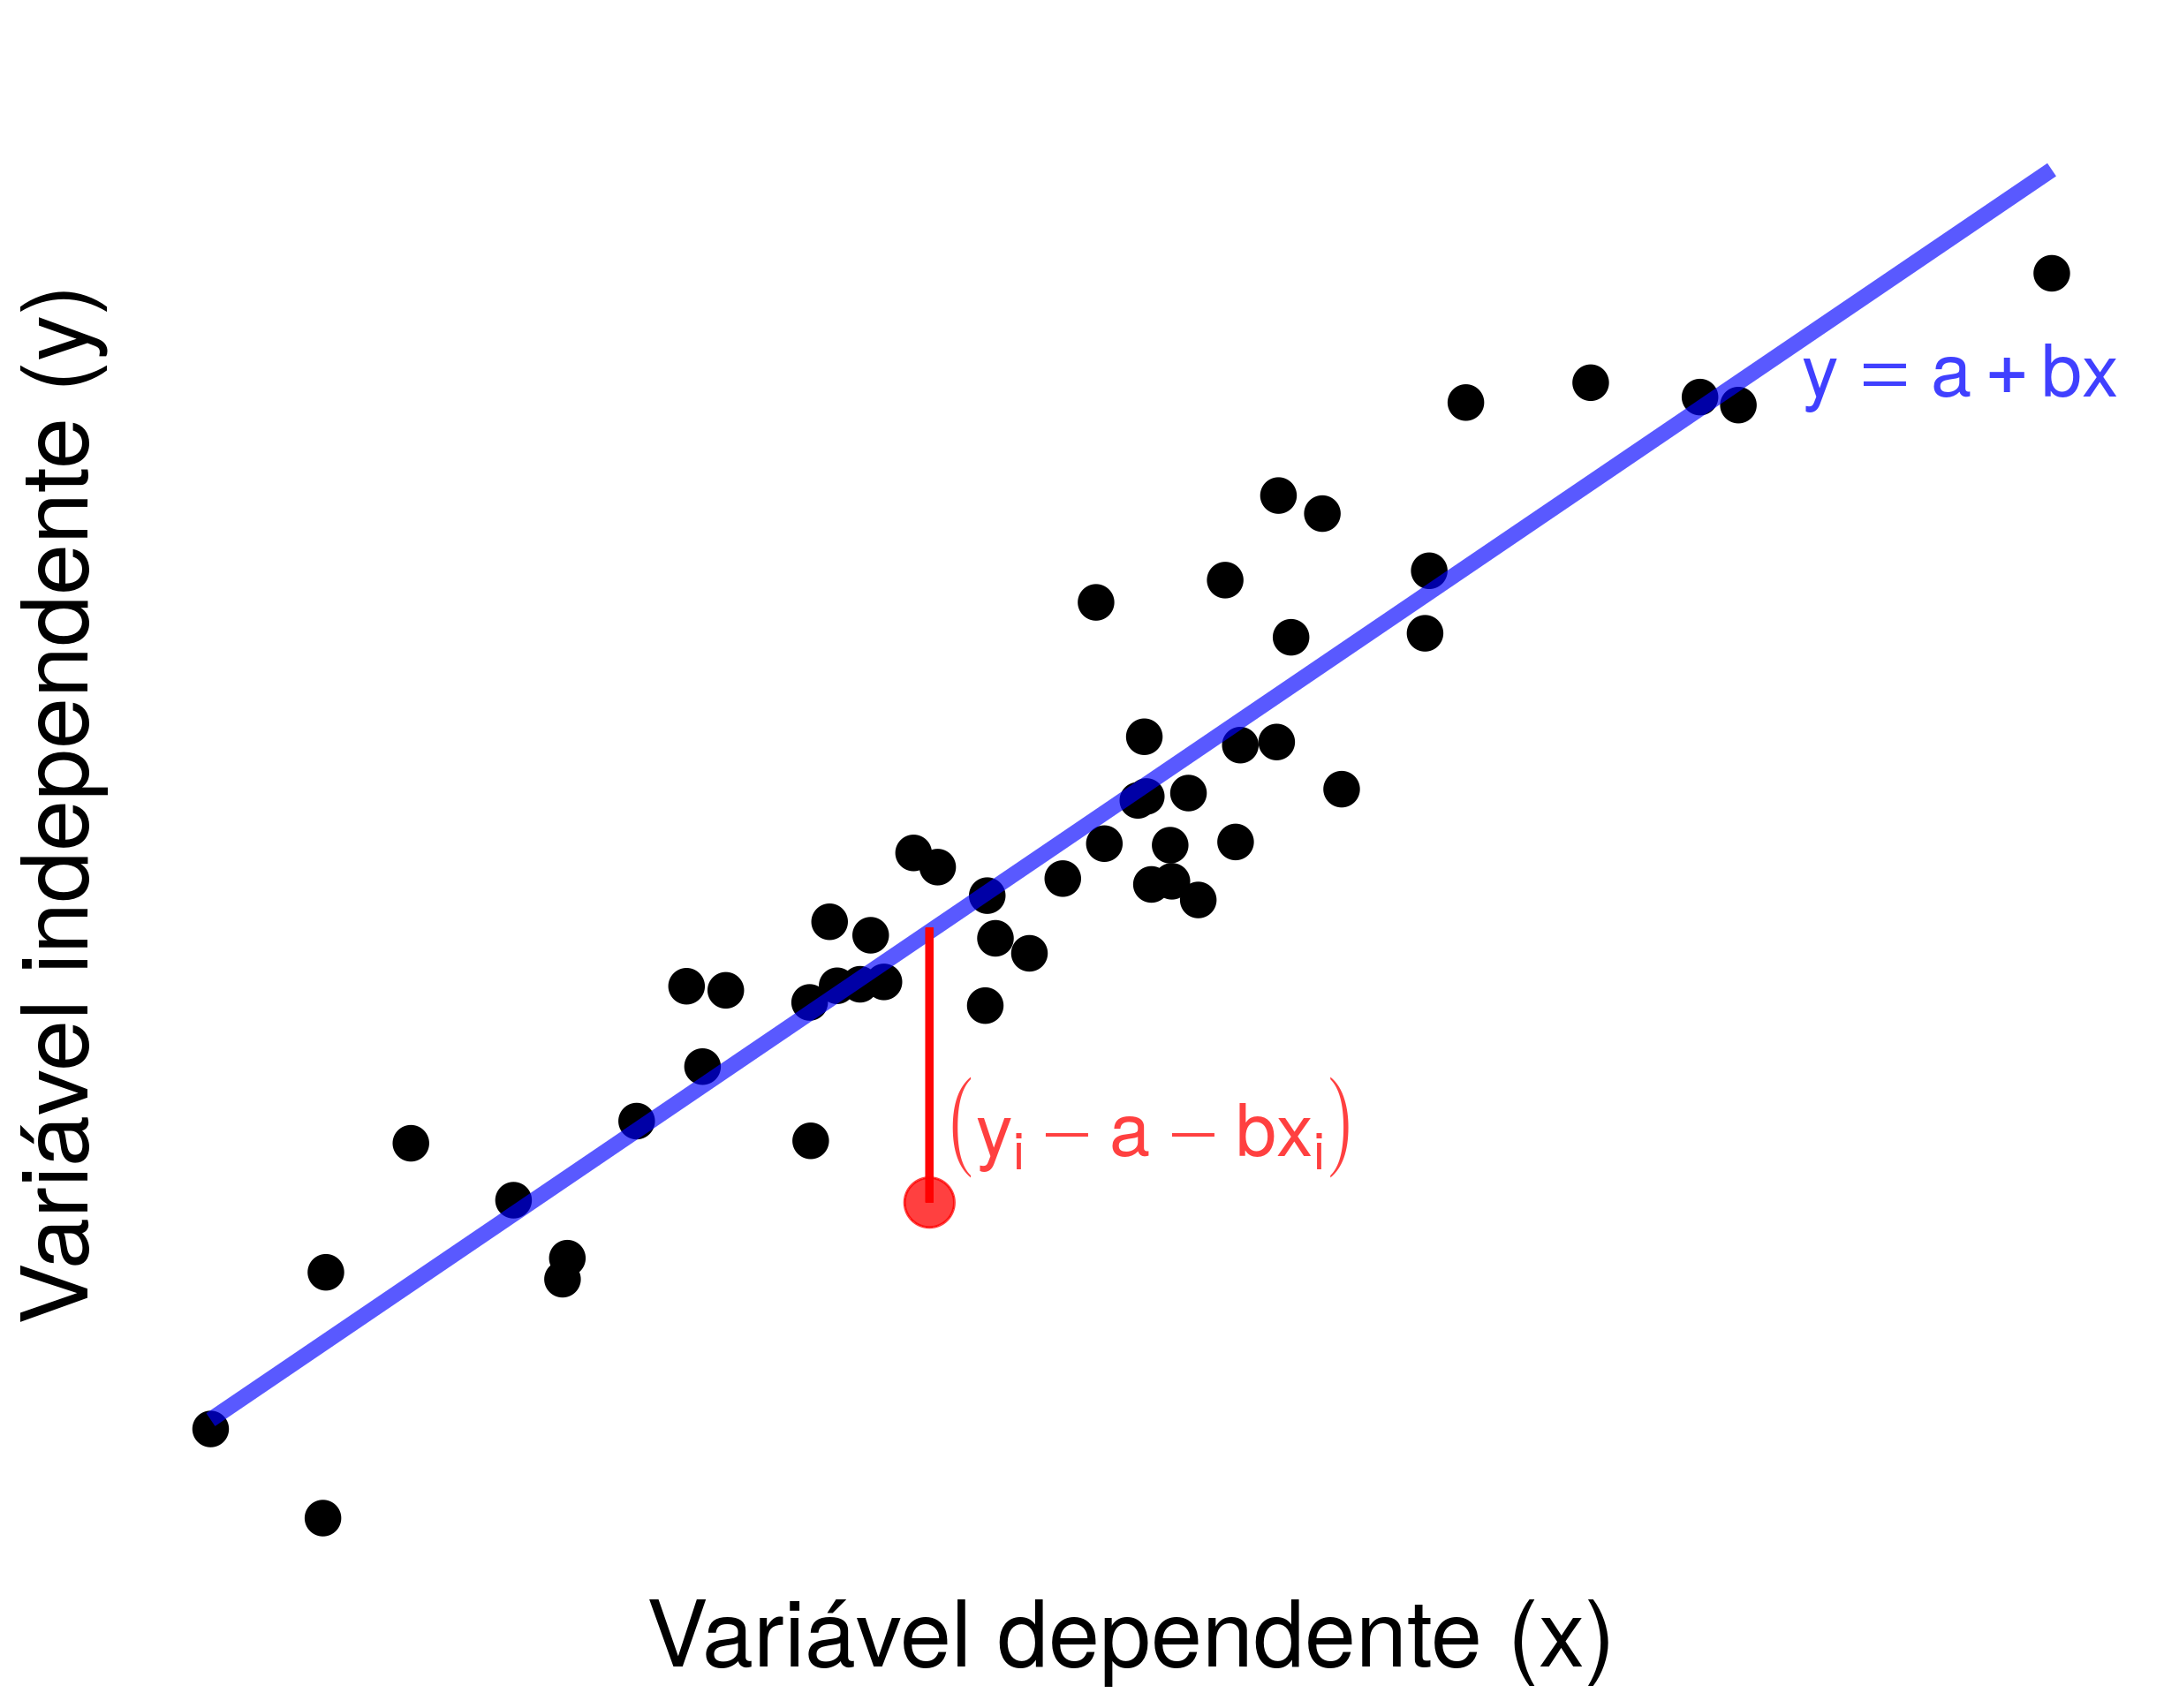
\includegraphics[width=6cm]{figure/motivacao_regressao.png}
	\end{figure}
\end{frame}

\subsection{Encontrando o intercepto e a inclinação}

\begin{frame}{Estimativas para $a$ e $b$}
	Imagine que temos $n$ observações da variável $X$ e $n$ observações da variável $Y$, conforme Tabela~\ref{tab:motivacao} e queremos encontrar a ``melhor reta'' como ilustrado na Figura~\ref{fig:motivacao}.

	
	O modelo de regressão linear simples é dado por
	\begin{align*}
	y_i = a + b \cdot x_i + \epsilon_i,\qquad i=1, \dots, n.
	\end{align*}
	
	O critério para determinar a ``melhor reta'' é denominado de \textcolor{blue}{Método dos Mínimos Quadrados} e consiste em encontrar $\hat{a}$ e $\hat{b}$ que minimiza a equação
	\begin{align*}
	S(a, b) &= (y_1 - a - bx_1)^2 + (y_2 - a - bx_2)^2+\cdots + (y_n - a - bx_n)^2.
	\end{align*}
	
	O ponto de mínimo $(\hat{a}, \hat{b})$ de $S(a,b)$ são soluções das seguintes equações:
	\begin{align} \label{eq:eq_normais}
	\nonumber&\dfrac{\partial S(\hat{a}, \hat{b})}{\partial a} =0\\
	&\dfrac{\partial S(\hat{a}, \hat{b})}{\partial b} =0
	\end{align}
\end{frame}

\begin{frame}{Regressão linear simples}
	
	{\scriptsize
	As estimativas de Mínimos Quadrados para o intercepto ($a$) e a inclinação ($b$) são
	\begin{align*}
		 \textcolor{red}{\hat{a}}\ &\textcolor{red}{=\bar{y}  - \hat{b} \cdot \bar{x}}\\
		\textcolor{red}{\hat{b}}\ &\textcolor{red}{= \dfrac{ S_{xy} - n \bar{x}\bar{y} }{S_{x^2} - n\bar{x}^2}}
	\end{align*}
	em que 
	\begin{table}
		\centering
		\begin{tabular}{l|l}
			 $S_{x} = x_1 + \dots + x_n$ & $S_{y} = y_1 + \dots + y_n$\\
			 $S_{xy} = x_1y_1 + x_2 y_2 + \dots + x_n y_n$ & $S_{x^2} = x_1^2 + x_2^2 + \dots + x_n^2$\\
			 $S_{y^2} = y_1^2 + y_2^2 + \dots + y_n^2$ & $S_{(x-\bar{x})^2} = (x_1 - \bar{x})^2 + \dots + (x_n - \bar{x})^2$ \\
			 $S_{(y-\bar{y})(x - \bar{x})} = (y_1 - \bar{y}) (x_1 - \bar{x}) + \dots + (y_n - \bar{y}) (x_n - \bar{x})$ & \\
		\end{tabular}
	\end{table}

	Além disso,
	\begin{align*}
		\bar{x} &= \frac{x_1 + x_2 + \dots +x_n }{n},\\
		\bar{y} &= \frac{y_1 + y_2 + \dots + y_n}{n},\\
		S_{(y-\bar{y})(x - \bar{x})} &= S_{xy} - n \bar{x} \bar{y} \\
		S_{(x-\bar{x})^2} &= S_{x^2} - n\bar{x}^2.
	\end{align*}
	\vfill
%	\begin{itemize}
%		\item $S_{x} = x_1 + \dots + x_n$;
%		\item $S_{y} = y_1 + \dots + y_n$;
%		\item $S_{xy} = x_1y_1 + x_2 y_2 + \dots + x_n y_n$;
%		\item $S_{x^2} = x_1^2 + x_2^2 + \dots + x_n^2$;
%		\item $S_{y^2} = y_1^2 + y_2^2 + \dots + y_n^2$;
%		\item $\bar{x} = \frac{x_1 + x_2 + \dots +x_n }{n}$;
%		\item $\bar{y} = \frac{y_1 + y_2 + \dots + y_n}{n}$.
%	\end{itemize}

	Note que a reta estimada é 
	\begin{align*}
		\hat{y} = \hat{a} + \hat{b}x,
	\end{align*}
	e para cada observação na amostra com $x_i$ e $y_i$, temos que a relação
	\begin{align*}
		y_i = \hat{a} + \hat{b}x_i + e_i, \quad i =1, \dots, n,
	\end{align*}
	em que $e_i = y_i - \hat{y}_i, \quad i =1, \dots, n$. Chamamos $e_i,\ i=1, \dots, n$ de resíduos.
}
\end{frame}

\begin{frame}{Propriedades da regressão linear simples}
	
\normalsize
	Esperamos que os resíduos são valores observados da variável erro $\epsilon \sim N(0, \sigma^2)$. Uma aproximação de $\sigma^2$   pode ser aproximada
	\begin{align*}
	\hat{\sigma}^2 = \dfrac{SQ_E}{n-2}
	\end{align*}
	em que 
	\begin{align*}
		SQ_E &= e_1^2 + \dots + e_n^2 = (y_1 - \hat{y}_1)^2 + \dots + (y_n - \hat{y}_n)^2=  S_{y^2} - n \bar{y}^2 -\hat{b} \left( S_{xy} - n \bar{x} \bar{y} \right).
	\end{align*}
	$SQ_E$ é chamado de Soma dos Quadrados dos Erros.
	
	Note que \textcolor{important}{ $\hat{b} \sim N\left(b;\vari(\hat{b}) = \frac{\sigma^2}{S_{(x-\bar{x})^2}}\right)$}  e \textcolor{important}{$\hat{a} \sim N\left(a; \vari(\hat{a}) = \sigma^2  \left[ \frac{1}{n} + \frac{\bar{x}^2}{s_{(x-\bar{x})^2}} \right] \right)$}.

E
\begin{align*}
\textcolor{red}{\dfrac{\hat{a} - a}{\sqrt{\widehat{\vari({\hat{a}})}}} \sim t_{n-2}}\qquad\qquad\qquad 
\textcolor{red}{\dfrac{\hat{b} - b}{\sqrt{\widehat{\vari({\hat{b}})}}} \sim t_{n-2}.}
\end{align*}
em que
\begin{align*}
\widehat{\vari({\hat{a}})} &= \hat\sigma^2 \left[  \frac{1}{n} + \frac{\bar{x}^2}{s_{(x-\bar{x})^2}} \right] =  \dfrac{ S_{y^2} - n \bar{y}^2 -\hat{b} \left( S_{xy} - n \bar{x} \bar{y} \right)}{n-2} \cdot \left[  \frac{1}{n} + \frac{\bar{x}^2}{s_{(x-\bar{x})^2}} \right],\\
\widehat{\vari({\hat{b}})} &= \frac{\hat\sigma^2}{S_{(x-\bar{x})^2}} = \dfrac{ S_{y^2} - n \bar{y}^2 -\hat{b} \left( S_{xy} - n \bar{x} \bar{y} \right)}{ (n - 2) \cdot  (S_{x^2} - n \bar{x}^2) }.
\end{align*}
\normalsize

\end{frame}

\subsection{Teste de hipóteses}

\begin{frame}{Teste de hipóteses para  a inclinação: $b$.}

Considere $n$ pares $(y_1, x_1), \dots, (y_n, x_n)$, e o modelo dado por
$$y_i = a + b \cdot x_i + \epsilon_i, \qquad i =1, \dots, n.$$
Considere o nível de significância $\alpha$.
\vfill

Queremos testar as seguintes hipóteses:
\begin{itemize}
	\item \textbf{Teste bilateral:} $H_0: b = b_0$ e $H_1: b \neq b_0$;
	\item \textbf{Teste unilateral:} $H_0: b \leq b_0$ e $H_1: b > b_0$;
	\item \textbf{Teste unilateral:} $H_0: b \geq b_0$ e $H_1: b < b_0$.
\end{itemize}
\vfill

\textbf{Ideia:} Primeiro calculamos a distância padronizada entre $b$ e $\hat{b}$: $T_0 = \frac{b - \hat{b}}{\sqrt{\widehat{\vari({\hat{b}})}}}$. Então,
\begin{itemize}
	\item \textbf{Teste bilateral:} Rejeitamos $H_0: b = b_0$ se $\lvert T_0 \rvert$ for grande;
	\item \textbf{Teste unilateral:} Rejeitamos $H_0: b \leq b_0$ se $ T_0 $ for grande;
	\item \textbf{Teste bilateral:} Rejeitamos $H_0: b \geq b_0$ se $T_0$ for pequeno.
\end{itemize}

\end{frame}

\begin{frame}{Teste de hipóteses para  a inclinação: $b$.}

\begin{figure}
	\centering
	\subfloat[Teste bilateral.]{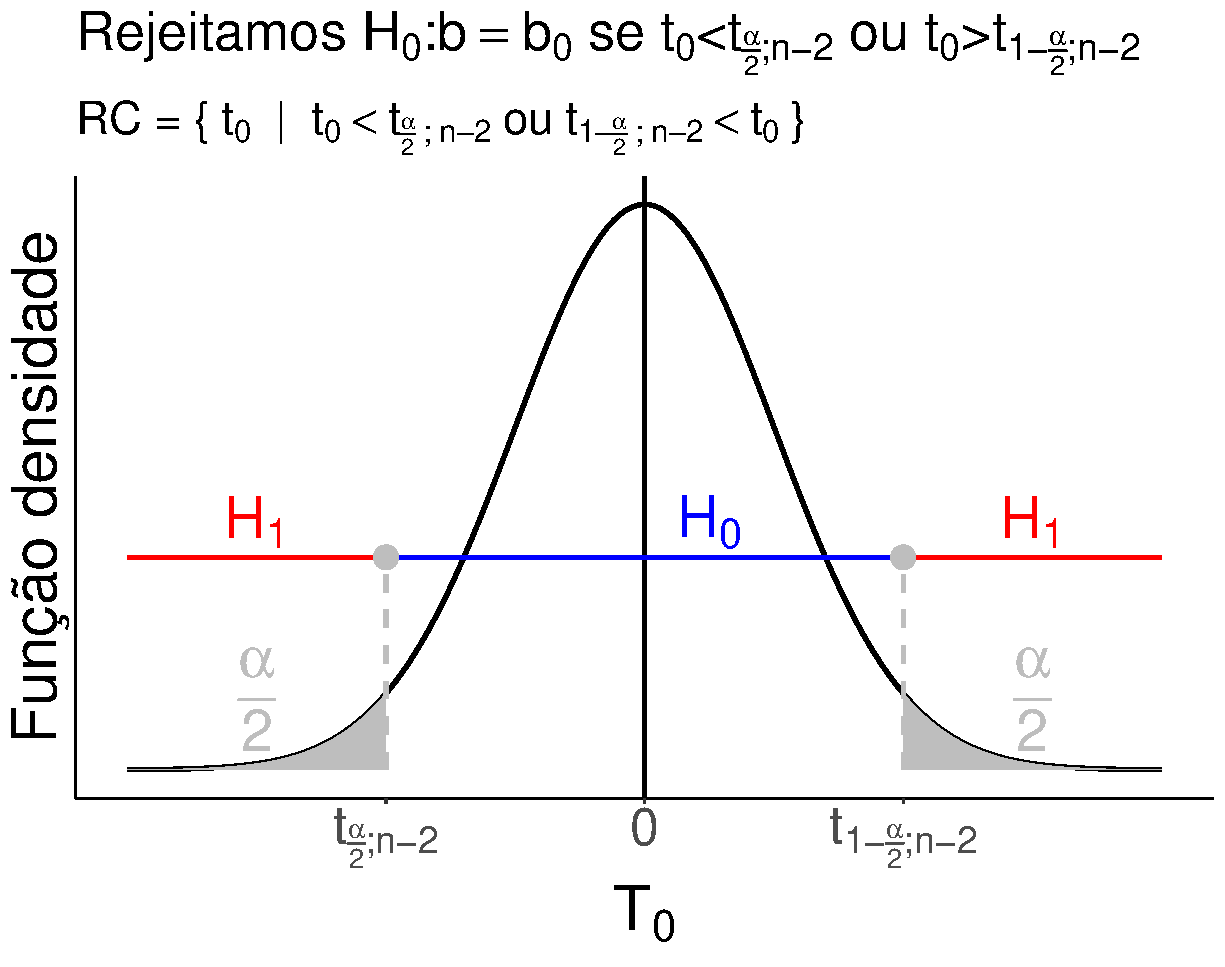
\includegraphics[width=0.315\linewidth]{figure/b-bilateral.pdf} \label{fig:b-bilateral}}
	\subfloat[Teste bilateral.]{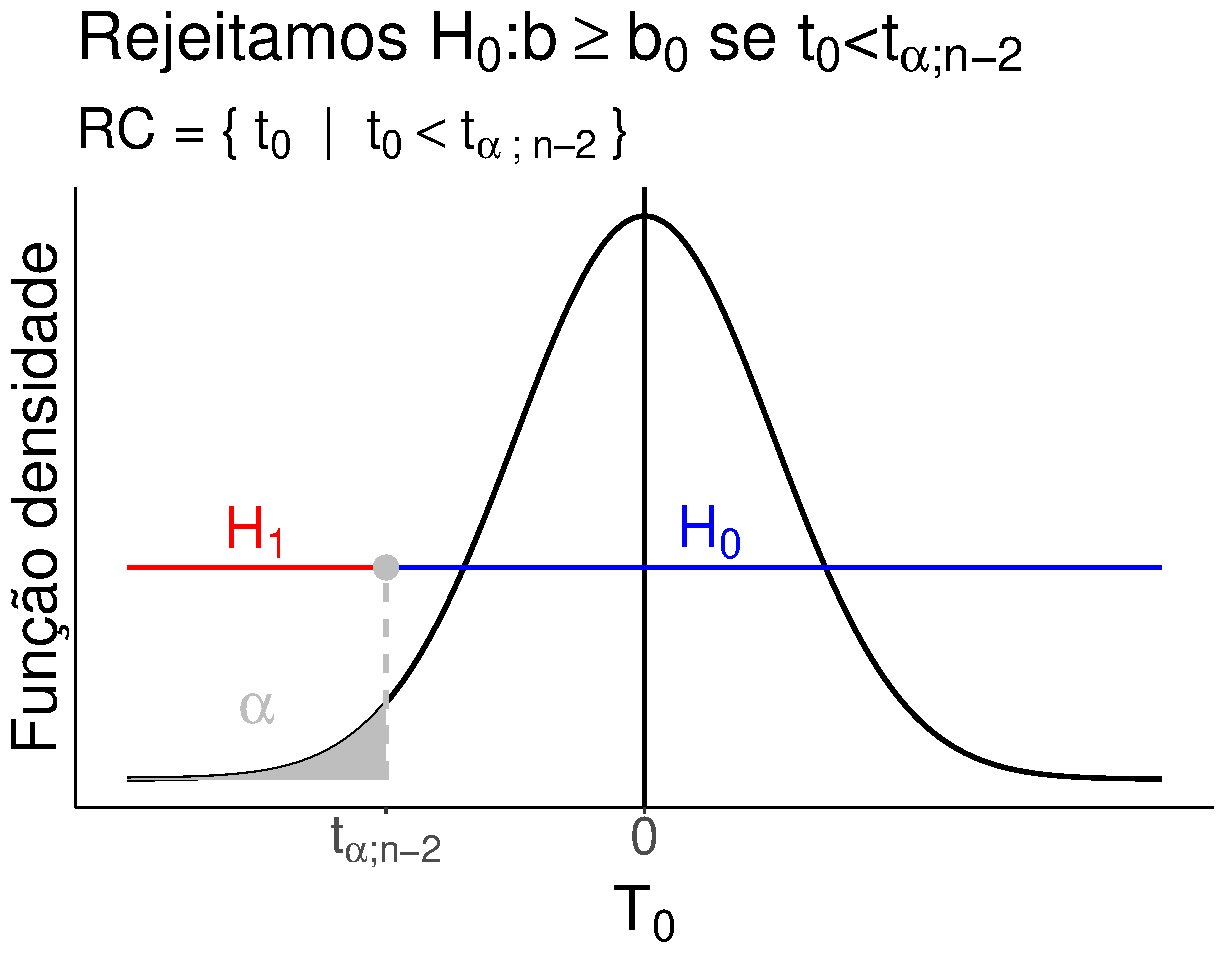
\includegraphics[width=0.315\linewidth]{figure/b-h1-lower.pdf} \label{fig:b-h1-lower}}
	\subfloat[Teste bilateral.]{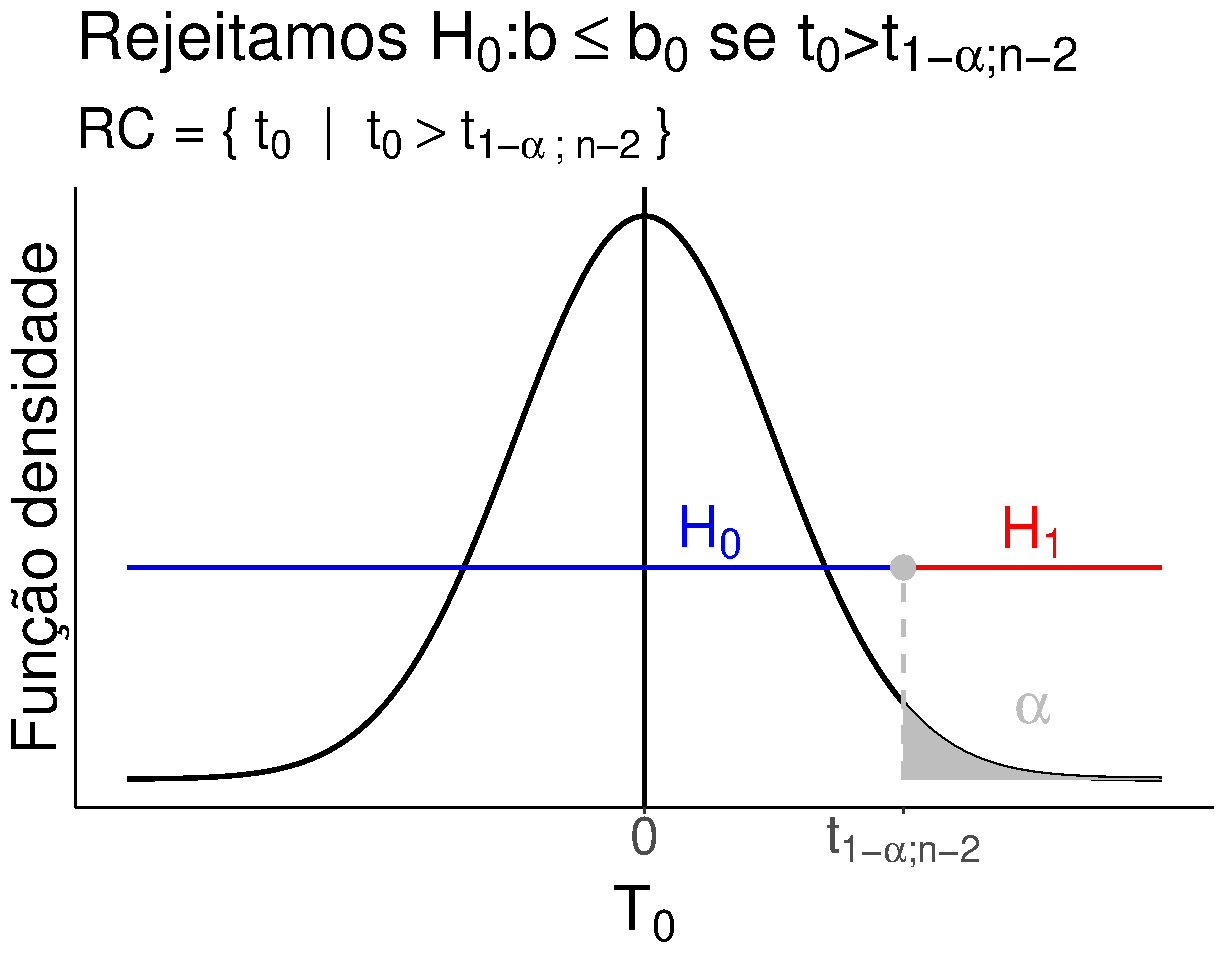
\includegraphics[width=0.315\linewidth]{figure/b-h1-upper.pdf} \label{fig:b-h1-upper}}
	\caption{Regiões críticas para testes sobre a inclinação $b$.}
\end{figure}

\end{frame}

\begin{frame}{Teste de hipóteses para  a inclinação: $b$.}

\begin{itemize}
	\item Na Figura~\ref{fig:b-bilateral}, testamos $H_0: b = b_0$ versus $H_1: b \neq b_0$. Rejeitamos $H_0$ se $t_0 = \frac{b  - \hat{b}}{\sqrt{\widehat{\vari({\hat{b}})}}} \allowbreak  \in RC = \left\{ t_0 \mid t_0 < t_{\frac{\alpha}{2};n-2}\mbox{ ou } t_{1-\frac{\alpha}{2}; n-2} < t_0 \right\}$, em que $P\left(t_{n-2} < t_{\frac{\alpha}{2},n-2}\right) = \frac{\alpha}{2}$ e $P\left(t_{n-2} < t_{1-\frac{\alpha}{2},n-2}\right) = 1-\frac{\alpha}{2}$;
	\vfill
	
	\item Na Figura~\ref{fig:b-h1-lower}, testamos $H_0: b \geq b_0$ versus $H_1: b < b_0$. Rejeitamos $H_0$ se $t_0 = \frac{b  - \hat{b}}{\sqrt{\widehat{\vari({\hat{b}})}}} \allowbreak  \in RC = \left\{ t_0 \mid t_0 < t_{\alpha;n-2} \right\}$, em que $P\left(t_{n-2} < t_{\alpha,n-2}\right) = \alpha$;
	\vfill
	
	\item Na Figura~\ref{fig:b-h1-upper}, testamos $H_0: b \leq b_0$ versus $H_1: b > b_0$. Rejeitamos $H_0$ se $t_0 = \frac{b  - \hat{b}}{\sqrt{\widehat{\vari({\hat{b}})}}} \allowbreak  \in RC = \left\{ t_0 \mid  t_{1-\alpha; n-2} < t_0 \right\}$, em que $P\left(t_{n-2} < t_{1-\alpha,n-2}\right) =1- \alpha$;
\end{itemize}

Chamamos $t_{\alpha; n-2}$, $t_{1-\alpha; n-2}$, $t_{\frac{\alpha}{2}; n-2}$ e $t_{1-\frac{\alpha}{2}; n-2}$ de valores críticos.

\end{frame}

\begin{frame}{Teste de hipóteses para  o intercepto: $a$.}

Considere $n$ pares $(y_1, x_1), \dots, (y_n, x_n)$, e o modelo dado por
$$y_i = a + b \cdot x_i + \epsilon_i, \qquad i =1, \dots, n.$$
Considere o nível de significância $\alpha$.
\vfill

Queremos testar as seguintes hipóteses:
\begin{itemize}
	\item \textbf{Teste bilateral:} $H_0: a = a_0$ e $H_1: a \neq a_0$;
	\item \textbf{Teste unilateral:} $H_0: a \leq a_0$ e $H_1: a > a_0$;
	\item \textbf{Teste unilateral:} $H_0: a \geq a_0$ e $H_1: a < a_0$.
\end{itemize}
\vfill

\textbf{Ideia:} Primeiro calculamos a distância padronizada entre $a$ e $\hat{a}$: $T_0 = \frac{a - \hat{a}}{\sqrt{\widehat{\vari({\hat{a}})}}}$. Então,
\begin{itemize}
	\item \textbf{Teste bilateral:} Rejeitamos $H_0: a = a_0$ se $\lvert T_0 \rvert$ for grande;
	\item \textbf{Teste unilateral:} Rejeitamos $H_0: a \leq a_0$ se $ T_0 $ for grande;
	\item \textbf{Teste bilateral:} Rejeitamos $H_0: a \geq a_0$ se $T_0$ for pequeno.
\end{itemize}

\end{frame}

\begin{frame}{Teste de hipóteses para  o intercepto: $a$.}

\begin{figure}
	\centering
	\subfloat[Teste bilateral.]{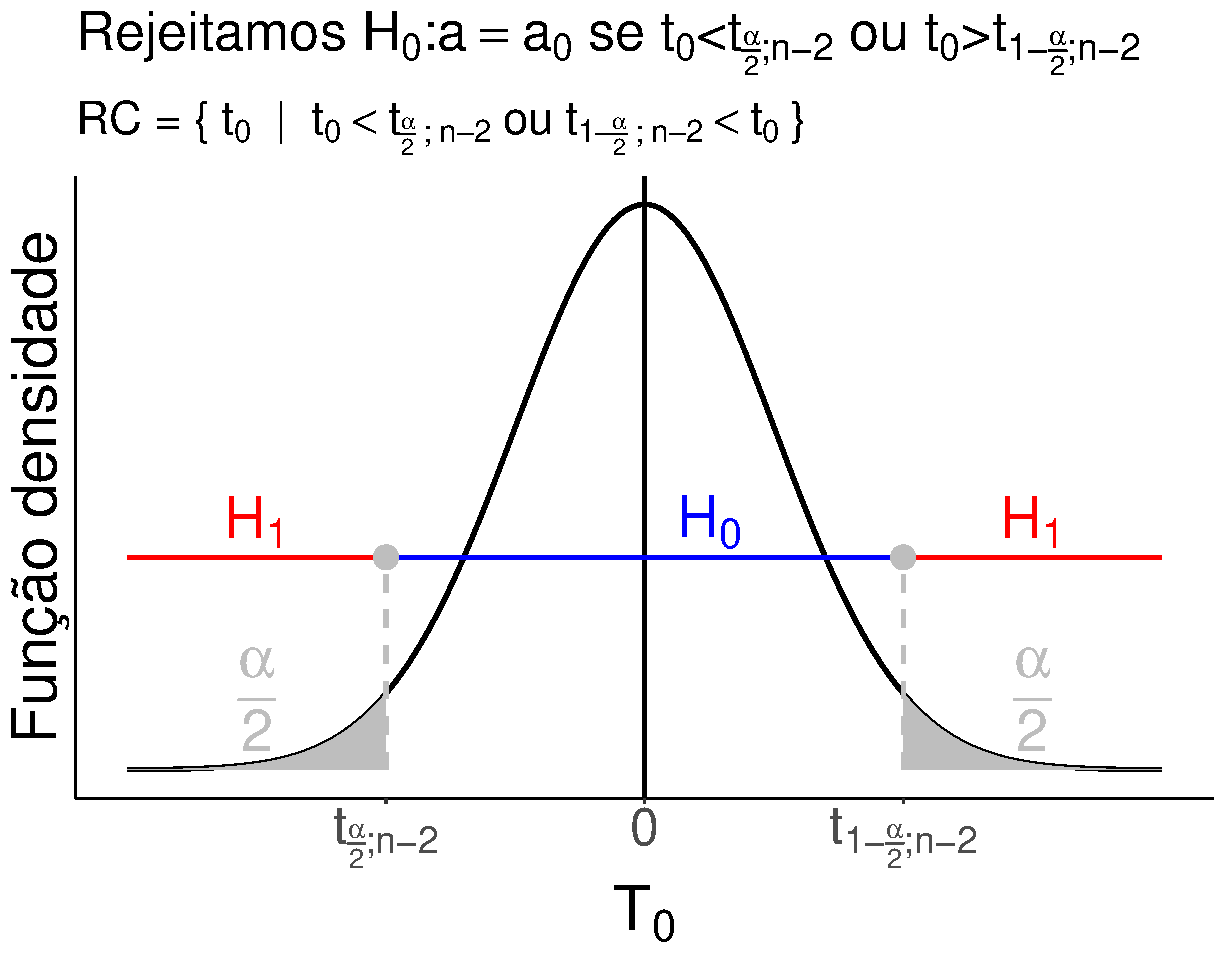
\includegraphics[width=0.315\linewidth]{figure/a-bilateral.pdf} \label{fig:a-bilateral}}
	\subfloat[Teste bilateral.]{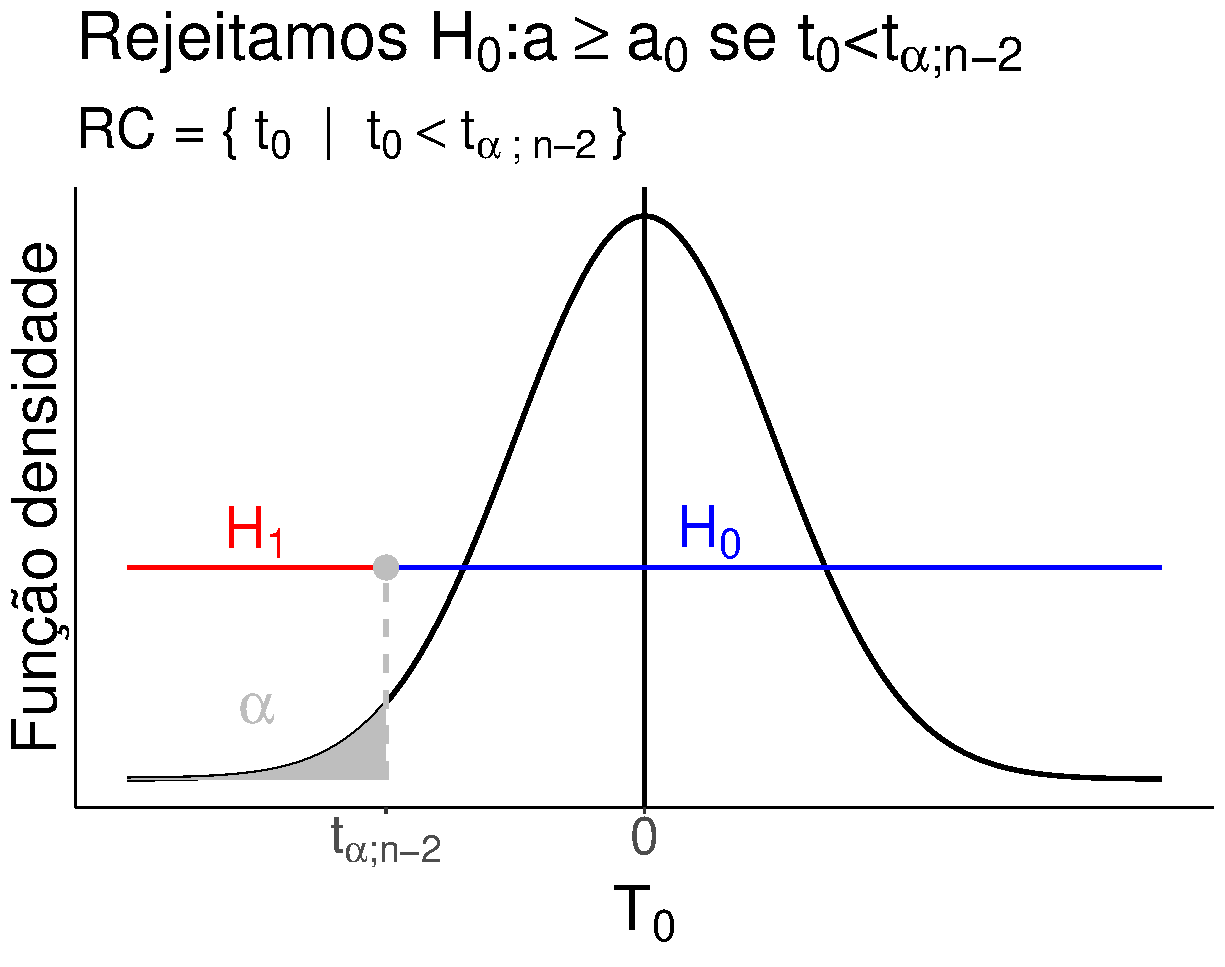
\includegraphics[width=0.315\linewidth]{figure/a-h1-lower.pdf} \label{fig:a-h1-lower}}
	\subfloat[Teste bilateral.]{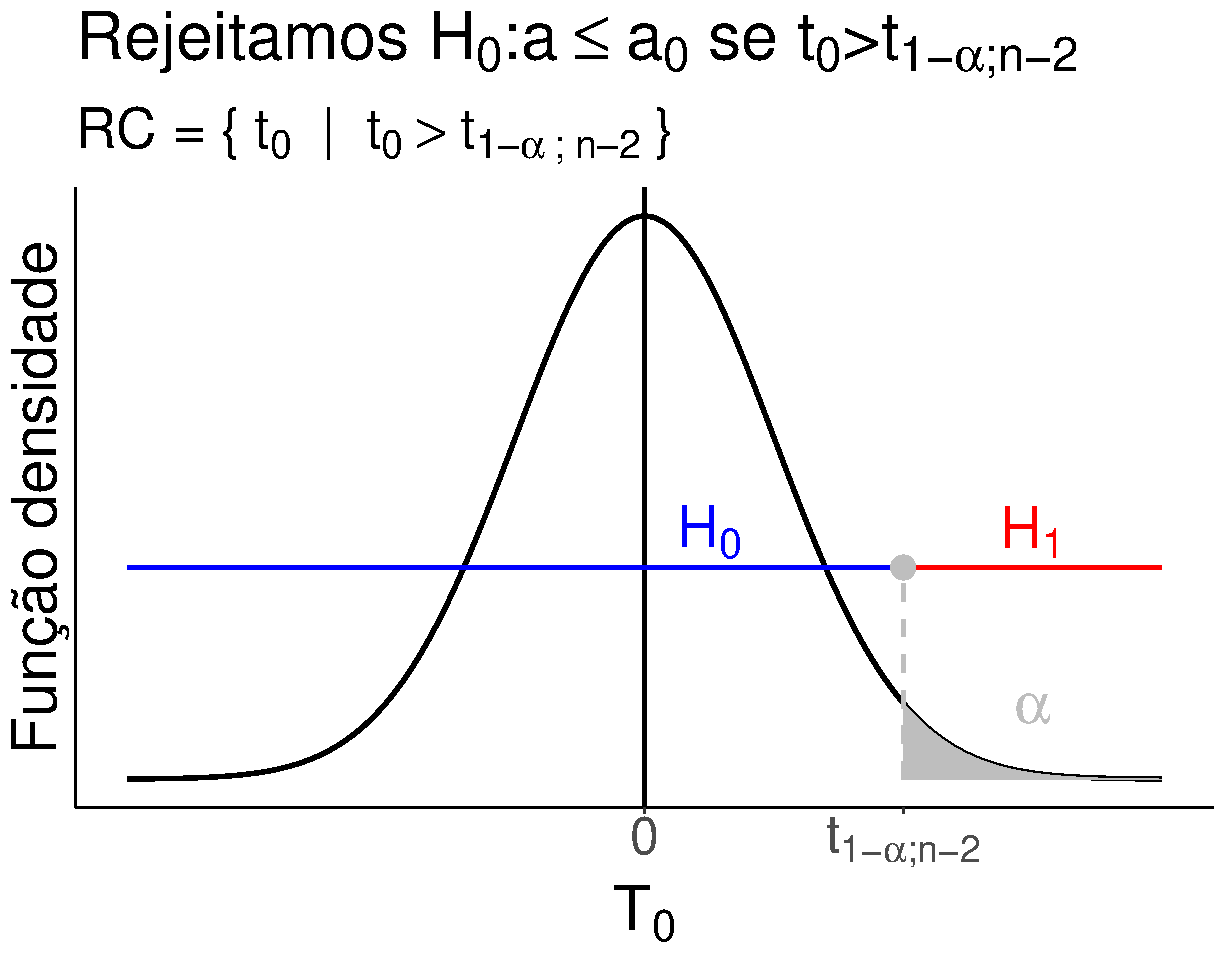
\includegraphics[width=0.315\linewidth]{figure/a-h1-upper.pdf} \label{fig:a-h1-upper}}
	\caption{Regiões críticas para testes sobre a inclinação $b$.}
\end{figure}

\end{frame}

\begin{frame}{Teste de hipóteses para o intercepto: $a$.}

\begin{itemize}
	\item Na Figura~\ref{fig:a-bilateral}, testamos $H_0: a = a_0$ versus $H_1: a \neq a_0$. Rejeitamos $H_0$ se $t_0 = \frac{a  - \hat{a}}{\sqrt{\widehat{\vari({\hat{a}})}}} \allowbreak  \in RC = \left\{ t_0 \mid t_0 < t_{\frac{\alpha}{2};n-2}\mbox{ ou } t_{1-\frac{\alpha}{2}; n-2} < t_0 \right\}$, em que $P\left(t_{n-2} < t_{\frac{\alpha}{2},n-2}\right) = \frac{\alpha}{2}$ e $P\left(t_{n-2} < t_{1-\frac{\alpha}{2},n-2}\right) = 1-\frac{\alpha}{2}$;
	\vfill
	
	\item Na Figura~\ref{fig:a-h1-lower}, testamos $H_0: a \geq a_0$ versus $H_1: a < a_0$. Rejeitamos $H_0$ se $t_0 = \frac{a  - \hat{a}}{\sqrt{\widehat{\vari({\hat{a}})}}} \allowbreak  \in RC = \left\{ t_0 \mid t_0 < t_{\alpha;n-2} \right\}$, em que $P\left(t_{n-2} < t_{\alpha,n-2}\right) = \alpha$;
	\vfill
	
	\item Na Figura~\ref{fig:a-h1-upper}, testamos $H_0: a \leq a_0$ versus $H_1: a > a_0$. Rejeitamos $H_0$ se $t_0 = \frac{a  - \hat{a}}{\sqrt{\widehat{\vari({\hat{a}})}}} \allowbreak  \in RC = \left\{ t_0 \mid  t_{1-\alpha; n-2} < t_0 \right\}$, em que $P\left(t_{n-2} < t_{1-\alpha,n-2}\right) =1- \alpha$;
\end{itemize}

Chamamos $t_{\alpha; n-2}$, $t_{1-\alpha; n-2}$, $t_{\frac{\alpha}{2}; n-2}$ e $t_{1-\frac{\alpha}{2}; n-2}$ de valores críticos.

\end{frame}



\subsection{Intervalo de confiança para o intercepto e a inclinação.}

\begin{frame}{Intervalo de confiança para o intercepto e a inclinação.}

\footnotesize
Considere $n$ pares $(y_1, x_1), \dots, (y_n, x_n)$, e o modelo dado por
$$y_i = a + b \cdot x_i + \epsilon_i, \qquad i =1, \dots, n.$$

\begin{block}{Intervalo de confiança para o intercepto: $a$.}
	Se o intercepto populacional é $a$, então $\frac{\hat{a} - a}{\sqrt{\widehat{\vari\left(\hat{a}\right)}}} \sim t_{n-2}$ e 
	$$\gamma = 1- \alpha = P \left( t_{\frac{\alpha}{2}; n-2} \leq \frac{\hat{a} - a}{\sqrt{\widehat{\vari\left(\hat{a}\right)}}} \leq t_{1-\frac{\alpha}{2}. n-2}  \right),$$
	e o intervalo de confiança para $a$ com coeficiente de confiança $\gamma = 1-\alpha$ é dado por
	$$IC(a, \gamma) =  \left( t_{\frac{\alpha}{2}; n-2} \sqrt{\widehat{\vari({\hat{a}})}} + \hat{a}; t_{1-\frac{\alpha}{2}; n-2} \sqrt{\widehat{\vari({\hat{a}})}} + \hat{a}  \right).$$
\end{block}

\begin{block}{Intervalo de confiança para a inclinação: $b$.}
	Se a inclinação populacional é $b$, então $\frac{\hat{b} - b}{\sqrt{\widehat{\vari\left(\hat{b}\right)}}} \sim t_{n-2}$ e 
	$$\gamma = 1- \alpha = P \left( t_{\frac{\alpha}{2}; n-2} \leq \frac{\hat{b} - b}{\sqrt{\widehat{\vari\left(\hat{b}\right)}}} \leq t_{1-\frac{\alpha}{2}. n-2}  \right),$$
	e o intervalo de confiança para $b$ com coeficiente de confiança $\gamma = 1- \alpha$ é dado por
	$$IC(b, \gamma) = \left( t_{\frac{\alpha}{2}; n-2} \sqrt{\widehat{\vari({\hat{b}})}} + \hat{b}; t_{1-\frac{\alpha}{2}; n-2} \sqrt{\widehat{\vari({\hat{b}})}} + \hat{b}  \right).$$
\end{block}
\normalsize

\end{frame}

\subsection{Intervalo de confiança para novas observações.}

\begin{frame}{Intervalo de confiança para o intercepto e a inclinação.}

\footnotesize
Considere $n$ pares $(y_1, x_1), \dots, (y_n, x_n)$, e o modelo dado por
$$y_i = a + b \cdot x_i + \epsilon_i, \qquad i =1, \dots, n.$$
Considere $x_0 \not\in \left\{ x_1, \dots, x_n \right\}$ e não conhecemos o valor de $Y_0 = a + b \cdot x_0 + \epsilon_0$.

\begin{block}{Estimativa pontual para $Y_0$.}
	Uma estimativa pontual para $Y_0$ é $\hat{y}_0 = \hat{a}  + \hat{b} \cdot x_0$. 
\end{block}

\begin{block}{Intervalo de confiança para $Y_0$.}
	Pode-se provar que 
	{\tiny
	$$\espe\left[Y_0 - \hat{Y}_0\right] = 0;  \vari\left[ Y_0 - \hat{Y}_0 \right] = \sigma^2 \left[ 1 + \frac{1}{n} + \frac{(x_0 - \bar{x})^2}{s_{(x-\bar{x})^2}} \right]; \frac{Y_0 - \hat{Y}_0}{ \sqrt{\hat{\sigma}^2 \left[ 1 + \frac{1}{n} + \frac{(x_0 - \bar{x})^2}{s_{(x-\bar{x})^2}} \right]}} \sim t_{n-2},$$
	}
	em que $\hat{\sigma}^2 = \frac{SQE}{n-2} = \frac{S_{y^2} -n \bar{y}^2 - \hat{b} (S_{xy} - n \bar{x} \bar{y})}{n-2}$. Então,
	{\tiny 
	$$\gamma = 1 - \alpha = P \left( t_{\frac{\alpha}{2}; n-2} \leq \frac{Y_0 - \hat{Y}_0}{\sqrt{\hat{\sigma}^2 \left[ 1 + \frac{1}{n} + \frac{(x_0 - \bar{x})^2}{s_{(x-\bar{x})^2}} \right]}} \leq t_{1-\frac{\alpha}{2}; n-2} \right),$$
	}
	e o intervalo de confiança para $Y_0$ com coeficiente de confiança $\gamma=1-\alpha$ é dado por
	{\tiny
	$$IC(Y_0, \gamma) = \left( t_{\frac{\alpha}{2}; n-2} \sqrt{\hat{\sigma}^2 \left[ 1 + \frac{1}{n} + \frac{(x_0 - \bar{x})^2}{s_{(x-\bar{x})^2}} \right]} + \hat{Y}_0 ; t_{1-\frac{\alpha}{2}; n-2} \sqrt{\hat{\sigma}^2 \left[ 1 + \frac{1}{n} + \frac{(x_0 - \bar{x})^2}{s_{(x-\bar{x})^2}} \right]} + \hat{Y}_0 \right).$$
	}
\end{block}
\normalsize

\end{frame}

\subsection{Análise de variância}

\begin{frame}{Análise de variância}

Considere $n$ pares $(y_1, x_1), \dots, (y_n, x_n)$, e o modelo dado por
$$y_i = a + b \cdot x_i + \epsilon_i, \qquad i =1, \dots, n.$$

Seja $\hat{y}_i = \hat{a} + \hat{b} x_i$ e $e_i = y_i - \hat{y}_i$. Então, pode-se provar que
\begin{align*}
\underbrace{\sum_{i=1}^{n} (y_i - \bar{y})^2} _{SQ_T = (n-1)s^2_y} = \underbrace{\sum_{i=1}^{n} (\hat{y}_i - \bar{y})^2 }_{SQ_R =\hat{b} S_{(x-\bar{x})(y - \bar{y})}} + \underbrace{\sum_{i=1}^{n} (\hat{y}_i - y_i)^2 }_{SQ_E = (n-1)s_e^2},
\end{align*}
em que 
\begin{itemize}
	\item $s^2_y = \frac{(y_1-\bar{y})^2 + (y_2-\bar{y})^2 + \cdots + (y_n-\bar{y})^2}{n-1}$;
	\item $s^2_e = \frac{(e_1-\bar{e})^2 + (e_2-\bar{e})^2 + \cdots + (e_n-\bar{e})^2}{n-1}$,  em que $\bar{e} = \frac{e_1 + \cdots + e_n}{n}$.
\end{itemize}

Pode-se provar que $\espe\left[SQ_R\right] = \sigma^2 + b^2 S_{(x-\bar{x})^2}$ e $\espe\left[ SQ_E \right] = (n-2)\sigma^2$. 

Considere $QM_E = \frac{SQ_E}{n-2}$ e $QM_R = \frac{SQ_R}{1}$. Se $H_0: b = 0$ é verdadeira, então $F_0 = \frac{QM_R}{QM_E} \sim F_{1, n-2}$.

De forma semelhante a ANOVA, chamamos: $SQ_T$ de soma de quadrados totais; $SQ_R$ de soma de quadrados de regressão; $SQ_E$ de soma de quadrados dos erros; $QM_R$ de quadrados médios de regressão; e $QM_E$ de quadrados médios dos erros.

\end{frame}

\begin{frame}{Análise de variância}

Imagine que desejamos decidir entre duas hipóteses: $H_0: b= 0$ e $H_1: b \neq 0$. Rejeitamos $H_0$ se $F_0$ for grande, e a rejeição crítica é dada por $RC = \left\{ f_0 \mid f_0 > f_{1-\alpha; 1, n-2} \right\}$. Na Figura~\ref{fig:anova-reg}, ilustramos esta região crítica.

\begin{figure}
	\centering
	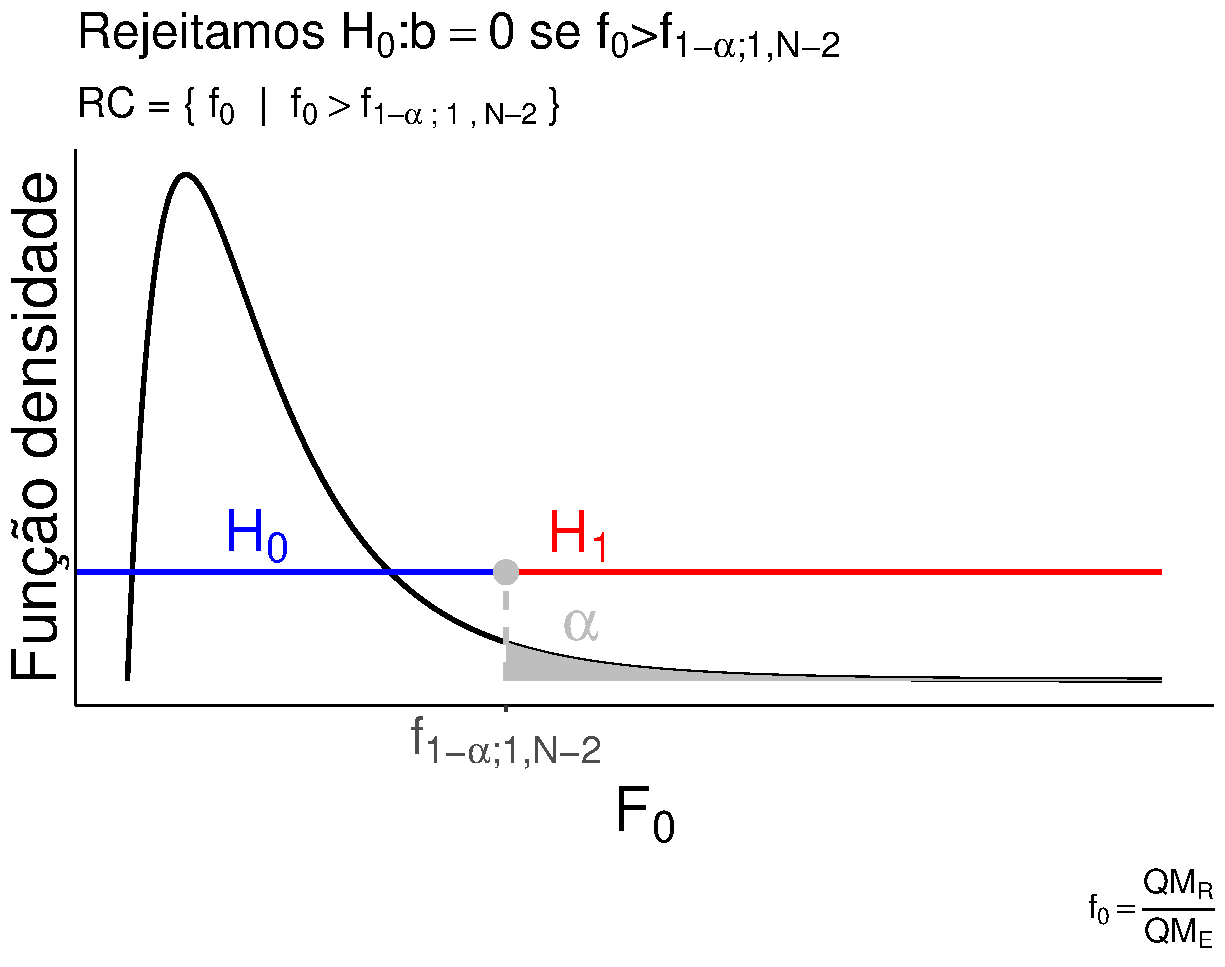
\includegraphics[width=0.65\linewidth]{figure/anova.pdf}
	\caption{Região para análise de variância para regressão linear simples.}
	\label{fig:anova-reg}
\end{figure}

\end{frame}

\subsection{Análise de resíduos.}

\begin{frame}{Checando as suposições do modelo matemática.}

\small
\begin{block}{Análise de resíduos.}
	Considere $n$ pares $(y_1, x_1), \dots, (y_n, x_n)$, e o modelo dado por
	$$y_i = a + b \cdot x_i + \epsilon_i, \qquad i =1, \dots, n.$$
	em que $\epsilon_i \in N(0, \sigma^2), i =1, \dots, n$. Chamamos $e_i = y_i - \hat{y}_i, i=1, \dots, n,$ de resíduos.

	Precisamos verificar se as seguintes suposições estão satisfeitas:
	\begin{enumerate}[(a)]
		\item \textbf{Linearidade:} para cada par $(x_i, e_i)$ desenhamos um ponto no plano cartesiano. Se não existe qualquer padrão e tendência, concluímos que a relação $y=a+b\cdot x$ captou toda influência de $x$ sobre $y$;
		\item \textbf{Normalidade:} para cada par $\left(q_{(i)}; \frac{e_{(i)} - \bar{e}}{s_e}\right)$ desenhamos um ponto no plano cartesiano, em que $\Phi(q_{(i)})  =\frac{i- 0,5}{n}, i=1, \dots, n$. Se os pontos estão sobre ou próximos da reta $y=x$, concluímos que as variáveis aleatórias $\epsilon_i, i=1, \dots, n,$ têm distribuição normal;
		\item \textbf{Independência:} para cada par $(i, d_i)$ desenhamos um ponto no plano cartesiano, em que $d_i = \frac{e_i}{\sqrt{\hat{\sigma}^2}}$ -- chamamos $d_i$ de resíduo padronizado. Se não existe padrão ou tendência, concluímos que as variáveis aleatórias $\epsilon_i$ são independentes;
		\item \textbf{Ponto exterior:} para cada par $(i, d_i)$ desenhamos um ponto no plano cartesiano, em que $d_i = \frac{e_i}{\sqrt{\hat{\sigma}^2}}$ -- chamamos $d_i$ de resíduo padronizado. Pontos abaixo de $-3$ ou acima de $3$ são pontos exteriores;
		\item \textbf{Igualdade da variância (homoscedasticidade):} para cada par $(e_i, \hat{y}_i)$ desenhamos um ponto no plano cartesiano. Se não existe padrão ou tendência, concluímos que as variáveis aleatórias $\epsilon_i$ tem a mesma variância.
	\end{enumerate}	
\end{block}
\normalsize

\end{frame}

\subsection{Exemplo}

\begin{frame}{Exemplo}

\normalsize

	Um motor de foguete é produzido por uma liga de dois tipos de propelentes: um iniciador e um mantenedor. Imagina-se que a força da liga $y$ é uma função linear da idade do propelente $x$ quando o motor é lançado. A Tabela~\ref{tab:propelente} fornece 20 observações. Estude a associação entre $X$ e $Y$. Ajuste uma regressão linear simples e verifique se a regressão linear é significativa. Qual a força da liga para um propelente com $20$ semanas (construa intervalo de confiança). Use $\alpha=5\%$ e $\gamma = 95\%$. 
	\vfill
	
	\begin{minipage}{0.45\linewidth}
		\begin{table}[ht]
			\centering
			\scalebox{0.5}{
			\begin{tabular}{cc}
				\toprule[0.05cm]
				Idade em semanas $(x)$ & Força $(y)$ \\ 
				\midrule[0.05cm]
				15,50 & 1823,01 \\ 
				23,75 & 1945,73 \\ 
				8,00 & 2446,80 \\ 
				17,00 & 2113,32 \\ 
				5,00 & 2512,34 \\ 
				19,00 & 1923,63 \\ 
				24,00 & 1676,79 \\ 
				2,50 & 2464,78 \\ 
				7,50 & 2463,42 \\ 
				11,00 & 2382,73 \\ 
				13,00 & 1999,45 \\ 
				3,75 & 2373,36 \\ 
				25,00 & 1754,28 \\ 
				9,75 & 2306,62 \\ 
				22,00 & 1735,37 \\ 
				18,00 & 1798,60 \\ 
				6,00 & 2545,93 \\ 
				12,50 & 2255,47 \\ 
				2,00 & 2459,01 \\ 
				21,50 & 1858,06 \\ 
				\bottomrule[0.05cm]
			\end{tabular}
			}
			\caption{Dados sobre propelentes de foguetes.} 
			\label{tab:propelente}
		\end{table}
	\end{minipage}	
	\begin{minipage}{0.45\linewidth}
		\begin{table}
			\centering
			\scalebox{0.5}{
			\begin{tabular}{l|l}
				$S_{x} =266,75	$ & $S_{y} = 42838,7	$\\
				$S_{xy} = 530297,5$ & $S_{x^2} = 4672,438$\\
				$S_{y^2} = 93550117$ & $S_{(x-\bar{x})^2} = 1114,659$ \\
				$S_{(y-\bar{y})(x - \bar{x})} = -41063,62$ & \\
			\end{tabular}
			}
		\end{table}
	\end{minipage}
	
\end{frame}

\begin{frame}{Exemplo}
	
\begin{block}{Solução -- diagrama de dispersão.}
	Na Figura~\ref{fig:exemplo-regressao}, $X$ (Idade em semanas) e $Y$ (força) estão negativamente e fortemente associadas.
	\begin{figure}[htbp]
		\centering
		\caption{Gráfico de dispersão.}
		\label{fig:exemplo-regressao}
		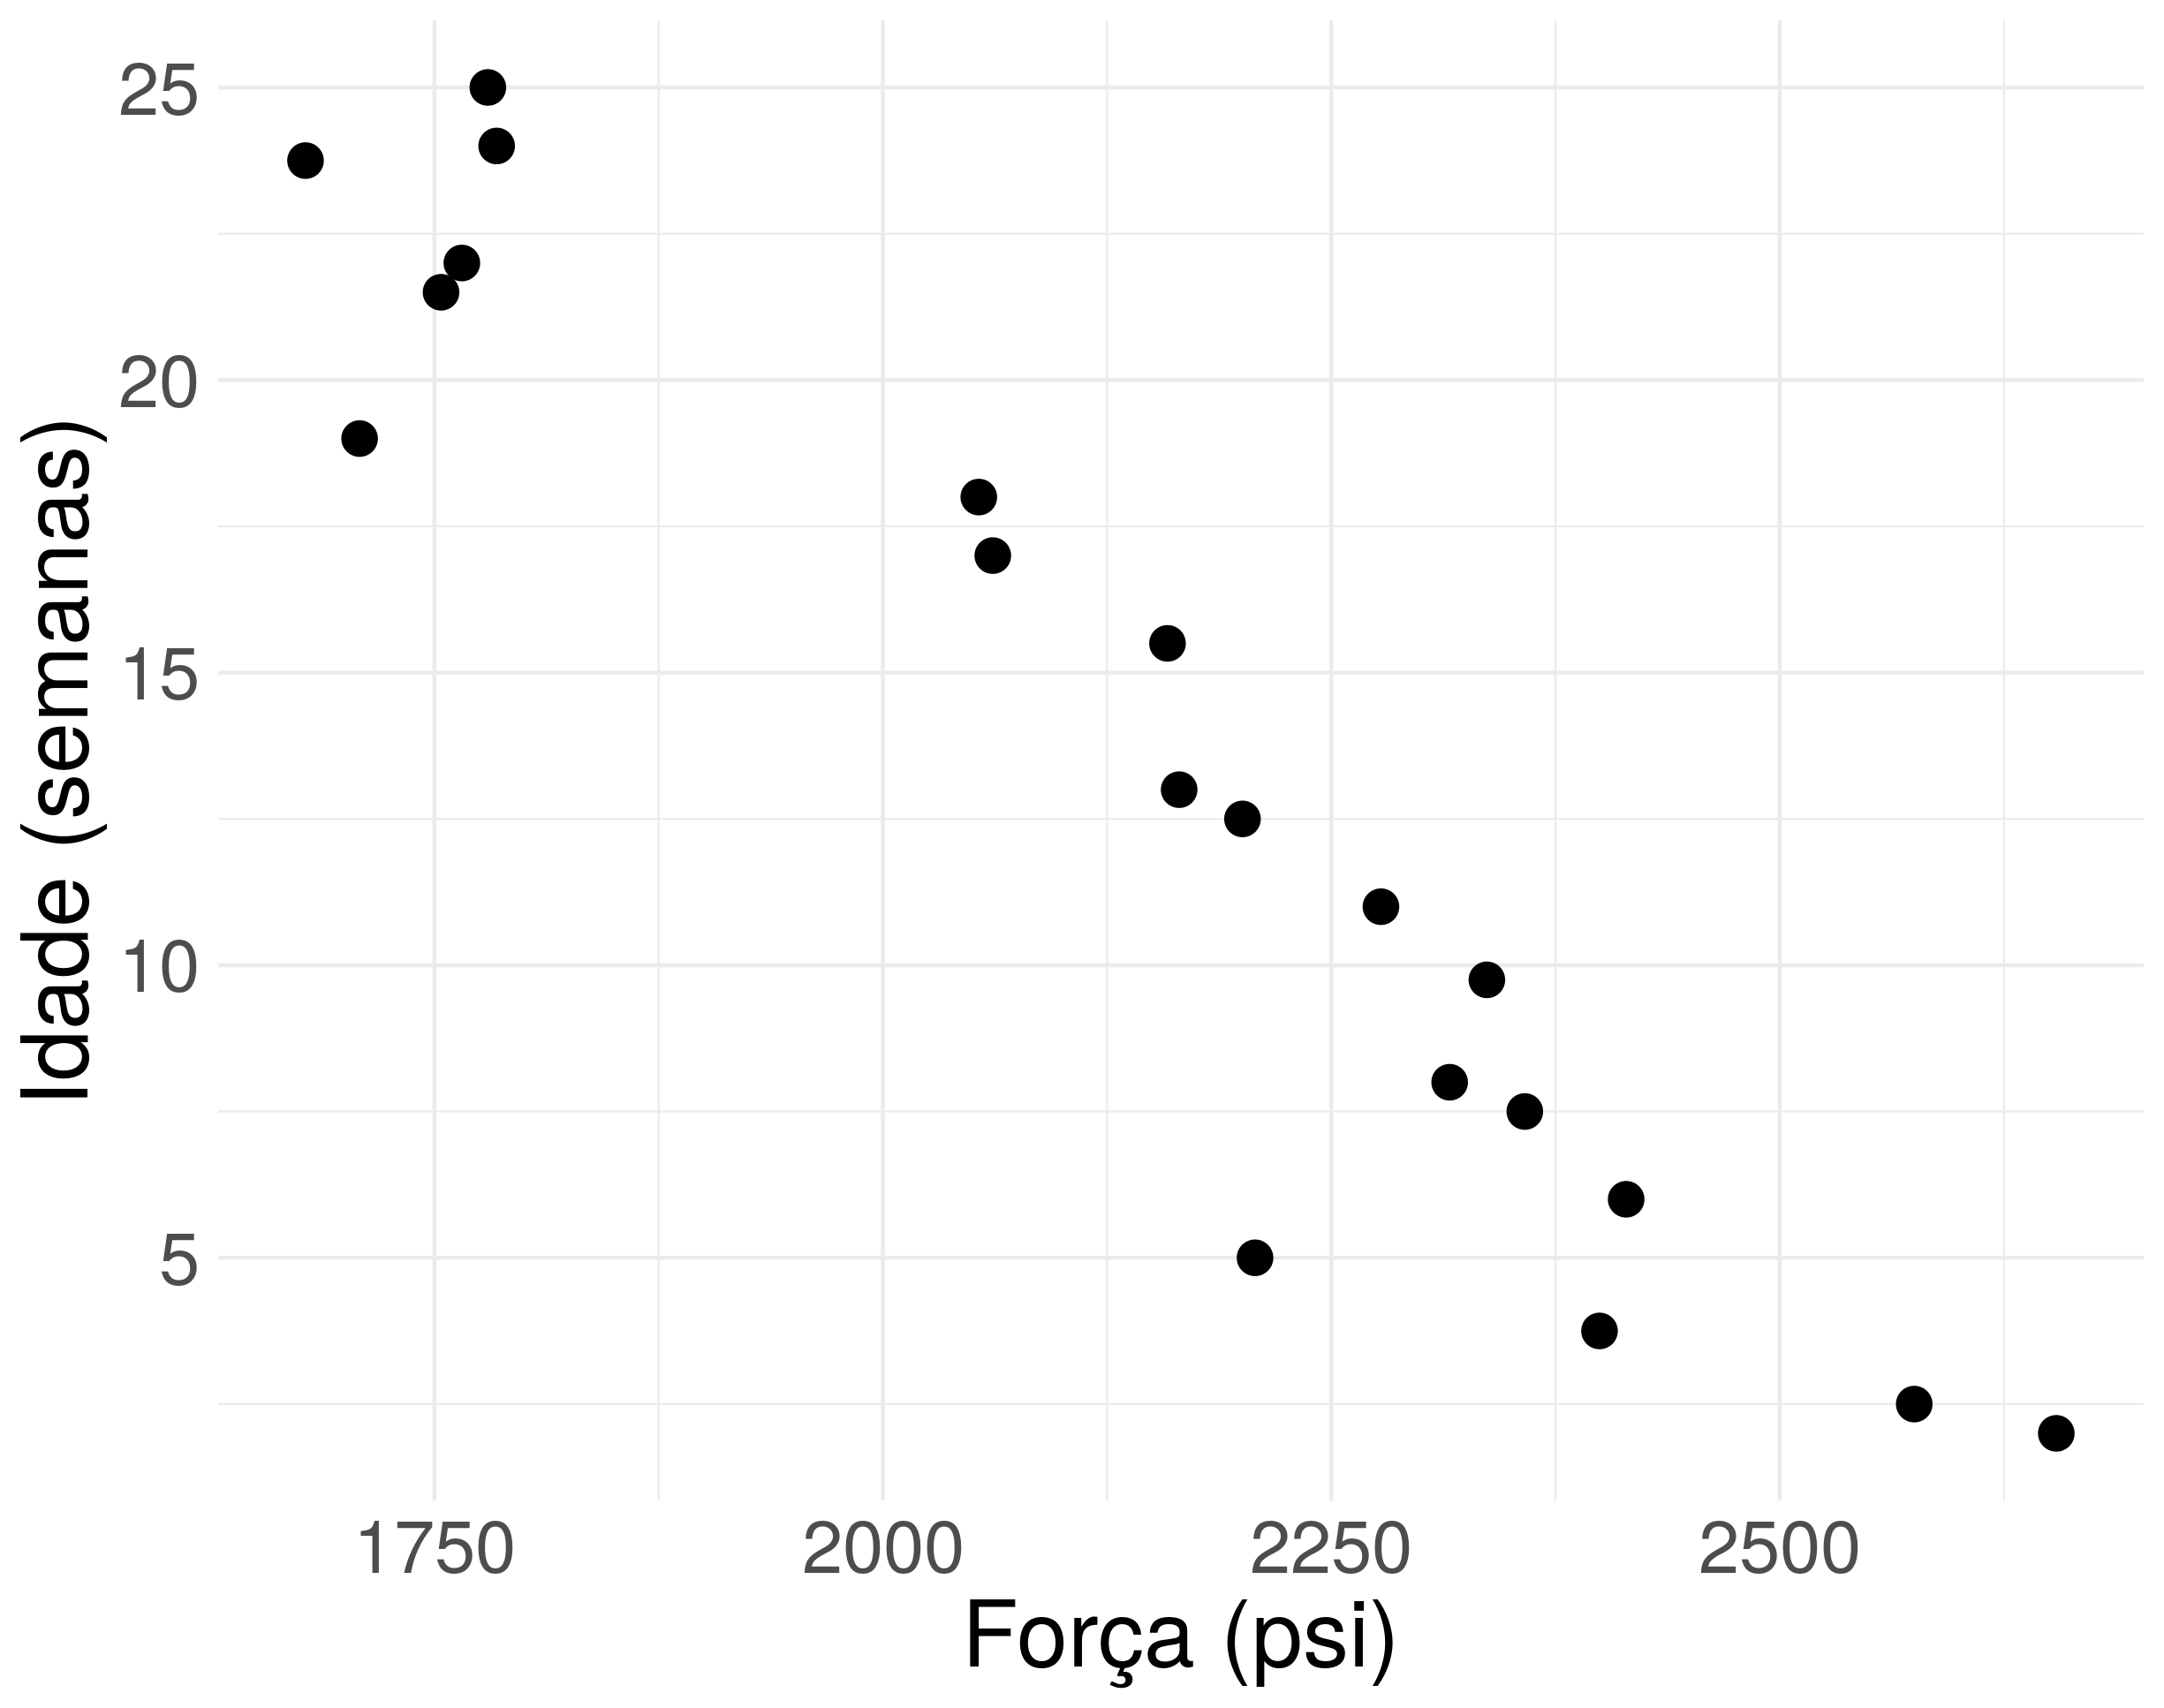
\includegraphics[width=0.5\linewidth]{figure/dispersao.png}
	\end{figure}
\end{block}

\end{frame}

\begin{frame}{Exemplo}
	
\small
	\begin{block}{Solução -- Ajuste da regressão linear}
		Nesse momento, queremos ajustar uma regressão linear simples, ou seja, queremos encontrar as estimativas $\hat{a}$ e $\hat{b}$ para o intercepto e para a inclinação da equação da reta.
		
		Primeiro vamos calcular a inclinação:
		\begin{align*}
		\hat{b} &= \dfrac{S_{x\cdot y} - n \bar{x} \bar{y}}{S_{x^2} - n \bar{x}^2},\\
		&= \dfrac{530297,5 - 20 \cdot 2141,935 \cdot 13,3375}{4672,438 - 20\cdot 13,3375	^2},\\
		&= -36,84.
		\end{align*}
		Agora podemos calcular o intercepto:
		\begin{align*}
		\hat{a} &= \bar{y} - \hat{b}\bar{x} = 2141,935	+ 36,84\cdot 13,3375\\
		&= 2633,28.
		\end{align*}		
		Finalmente, vamos estimar a variância do erro:
		\begin{align*}
		\hat{\sigma}^2 &= SQE = S_{y^2} - n \bar{y}^2 - \hat{b}(S_{xy} - n \bar{x} \bar{y}) \\
		&= 93550117 - 20 \cdot \left(\frac{42838,7}{20}\right)^2 - (-36,84)\cdot \left(530297,5 - 20 \cdot \frac{266,75}{20} \frac{42838,7}{20}\right)\\
		&= 9811,212.
		\end{align*}
	\end{block}
\normalsize
	
\end{frame}


\begin{frame}{Exemplo}

	\begin{block}{Solução -- teste de hipóteses}
		Vamos decidir entre as hipóteses: $H_0: b=0$ e $H_1: b \neq 0$.
		
		\textbf{Passo 1)} Queremos decidir entre as hipóteses: $H_0: b = 0$  e $H_1: b \neq 0$;
		
		\textbf{Passo 2)} Nível de significância $\alpha=5\%$;
		
		\textbf{Passo 3)} Rejeitamos $H_0$ se $\lvert T_0 \rvert = \left\lvert \frac{b - \hat{b}}{\sqrt{\widehat{\vari({\hat{b}})}}} \right\rvert$ for grande. Ou seja, $RC = \left\{ t_0 \mid t_0 < t_{\frac{\alpha}{2}; n-2} \mbox{ ou } t_0 < t_{1-\frac{\alpha}{2}; n-2}  \right\}$;
		
		\textbf{Passo 4)} Vamos encontrar o valor crítico:
		\begin{itemize}
			\item $P\left(t_{n-2} \leq t_{\frac{\alpha}{2}; n-2}\right) = P\left(t_{28} \leq t_{0,025; 18}\right) = \frac{\alpha}{2} = 0,025$, então $t_{0,025; 18} =  -2,101
			$;
			\item $P\left(t_{n-2} \leq t_{1-\frac{\alpha}{2}; n-2}\right) = P\left(t_{28} \leq t_{0,975; 18}\right) = 1-\frac{\alpha}{2} = 0,975$, então $t_{0,975; 18} =  2,101
			$;
		\end{itemize}
	
		\textbf{Passo 5)} Note que $\hat{b} = -36,84$, $\widehat{\vari({\hat{b}})} = \frac{\hat{\sigma}^2}{S_{(x-\bar{x})^2}} = \frac{9811,212}{1114,659} = 8,80$ e $t_0 = \frac{-36,84 - 0}{\sqrt{8,80}} = -12,42 \in RC$, e rejeitamos $H_0$.
		
		Ao nível de significância $\alpha=5\%$, a inclinação populacional na regressão linear simples $b$ é diferente de zero.
	\end{block}


\end{frame}

\begin{frame}{Exemplo}

	\begin{block}{Solução -- teste de hipóteses}
	Vamos decidir entre as hipóteses: $H_0: a=0$ e $H_1: a \neq 0$.
	
	\textbf{Passo 1)} Queremos decidir entre as hipóteses: $H_0: a = 0$  e $H_1: a \neq 0$;
	
	\textbf{Passo 2)} Nível de significância $\alpha=5\%$;
	
	\textbf{Passo 3)} Rejeitamos $H_0$ se $\lvert T_0 \rvert = \left\lvert \frac{a - \hat{a}}{\sqrt{\widehat{\vari({\hat{a}})}}} \right\rvert$ for grande. Ou seja, $RC = \left\{ t_0 \mid t_0 < t_{\frac{\alpha}{2}; n-2} \mbox{ ou } t_0 < t_{1-\frac{\alpha}{2}; n-2}  \right\}$;
	
	\textbf{Passo 4)} Vamos encontrar o valor crítico:
	\begin{itemize}
		\item $P\left(t_{n-2} \leq t_{\frac{\alpha}{2}; n-2}\right) = P\left(t_{28} \leq t_{0,025; 18}\right) = \frac{\alpha}{2} = 0,025$, então $t_{0,025; 18} =  -2,101
		$;
		\item $P\left(t_{n-2} \leq t_{1-\frac{\alpha}{2}; n-2}\right) = P\left(t_{28} \leq t_{0,975; 18}\right) = 1-\frac{\alpha}{2} = 0,975$, então $t_{0,975; 18} =  2,101
		$;
	\end{itemize}
	
	\textbf{Passo 5)} Note que $\hat{a} = 2633,28$, $\bar{x} = \frac{S_x}{n} = \frac{266,75}{20} = 13,34$,  $\widehat{\vari({\hat{a}})} = \hat{\sigma}^2 \left[ \frac{1}{n} +  \frac{\bar{x}^2}{S_{(x-\bar{x})^2}} \right] =  9811,212 \left[ \frac{1}{20} + \frac{13,34^2}{11114,659} \right]  = 2056,923$ e $t_0 = \frac{a - \hat{a}}{\sqrt{\widehat{\vari({\hat{a}})}}} = \frac{2633,28 - 0}{\sqrt{2056,923}} = 58,06  \in RC$, e rejeitamos $H_0$.
	
	Ao nível de significância $\alpha=5\%$, o intercepto populacional na regressão linear simples $a$ é diferente de zero.
\end{block}
\end{frame}

\begin{frame}{Exemplo}

\begin{block}{Intervalo de confiança para o intercepto: $a$.}
	Note que $\hat{a} = 2633,28$ e $\widehat{\vari({\hat{a}})} = 2056,923$. Vamos usar o coeficiente de confiança $\gamma = 1 - \alpha = 95\%$ e $\alpha=5\%$.
	
	Primeiro vamos encontrar os quantis da distribuição $t$-Student:
	\begin{itemize}
		\item $P(t_{n-2} \leq t_{\frac{\alpha}{2};n-2}) = P(t_{18} \leq t_{0,025; 18}) = \frac{\alpha}{2} = 0,025$, então $t_{0,025; 18} = -2,101$;
		\item $P(t_{n-2} \leq t_{1-\frac{\alpha}{2};n-2}) = P(t_{18} \leq t_{0,975; 18}) = 1-\frac{\alpha}{2} = 0,975$, então $t_{0,975; 18} = 2,101$.
	\end{itemize}
	Então o intervalo de confiança para o intercepto com coeficiente de confiança $\gamma = 0,95$ é dado por
	\begin{align*}
		IC\left(a;95\%\right) &= \left( t_{\frac{\alpha}{2};n-2} \sqrt{\widehat{\vari({\hat{a}})}} + \hat{a}; t_{1-\frac{\alpha}{2};n-2} \sqrt{\widehat{\vari({\hat{a}})}} + \hat{a} \right)\\
		&= \left( -2,101 \cdot \sqrt{2056,923} + 2633,28; 2,101 \cdot \sqrt{2056,923} + 2633,28 \right)\\
		&=  \left( 2537,993; 2728,567 \right)
	\end{align*}
\end{block}

\end{frame}

\begin{frame}{Exemplo}

\begin{block}{Intervalo de confiança para a inclinação: $b$.}
	Note que $\hat{b} = -36,84$ e $\widehat{\vari({\hat{b}})} = 8,80$. Vamos usar o coeficiente de confiança $\gamma = 1 - \alpha = 95\%$ e $\alpha=5\%$.
	
	Primeiro vamos encontrar os quantis da distribuição $t$-Student:
	\begin{itemize}
		\item $P(t_{n-2} \leq t_{\frac{\alpha}{2};n-2}) = P(t_{18} \leq t_{0,025; 18}) = \frac{\alpha}{2} = 0,025$, então $t_{0,025; 18} = -2,101$;
		\item $P(t_{n-2} \leq t_{1-\frac{\alpha}{2};n-2}) = P(t_{18} \leq t_{0,975; 18}) = 1-\frac{\alpha}{2} = 0,975$, então $t_{0,975; 18} = 2,101$.
	\end{itemize}
	Então o intervalo de confiança para a inclinação com coeficiente de confiança $\gamma = 0,95$ é dado por
	\begin{align*}
	IC\left(b;95\%\right) &= \left( t_{\frac{\alpha}{2};n-2} \sqrt{\widehat{\vari({\hat{b}})}} + \hat{b}; t_{1-\frac{\alpha}{2};n-2} \sqrt{\widehat{\vari({\hat{b}})}} + \hat{b} \right)\\
	&= \left( -2,101 \cdot \sqrt{8,80} -36,84; 2,101 \cdot \sqrt{8,80} -36,84 \right)\\
	&=  \left( -43,07; -30,61 \right)
	\end{align*}
\end{block}

\end{frame}

\begin{frame}{Exemplo}

\begin{block}{Solução -- análise de resíduos}
	\begin{figure}
		\centering
		\subfloat[Homoscedasticidade.]{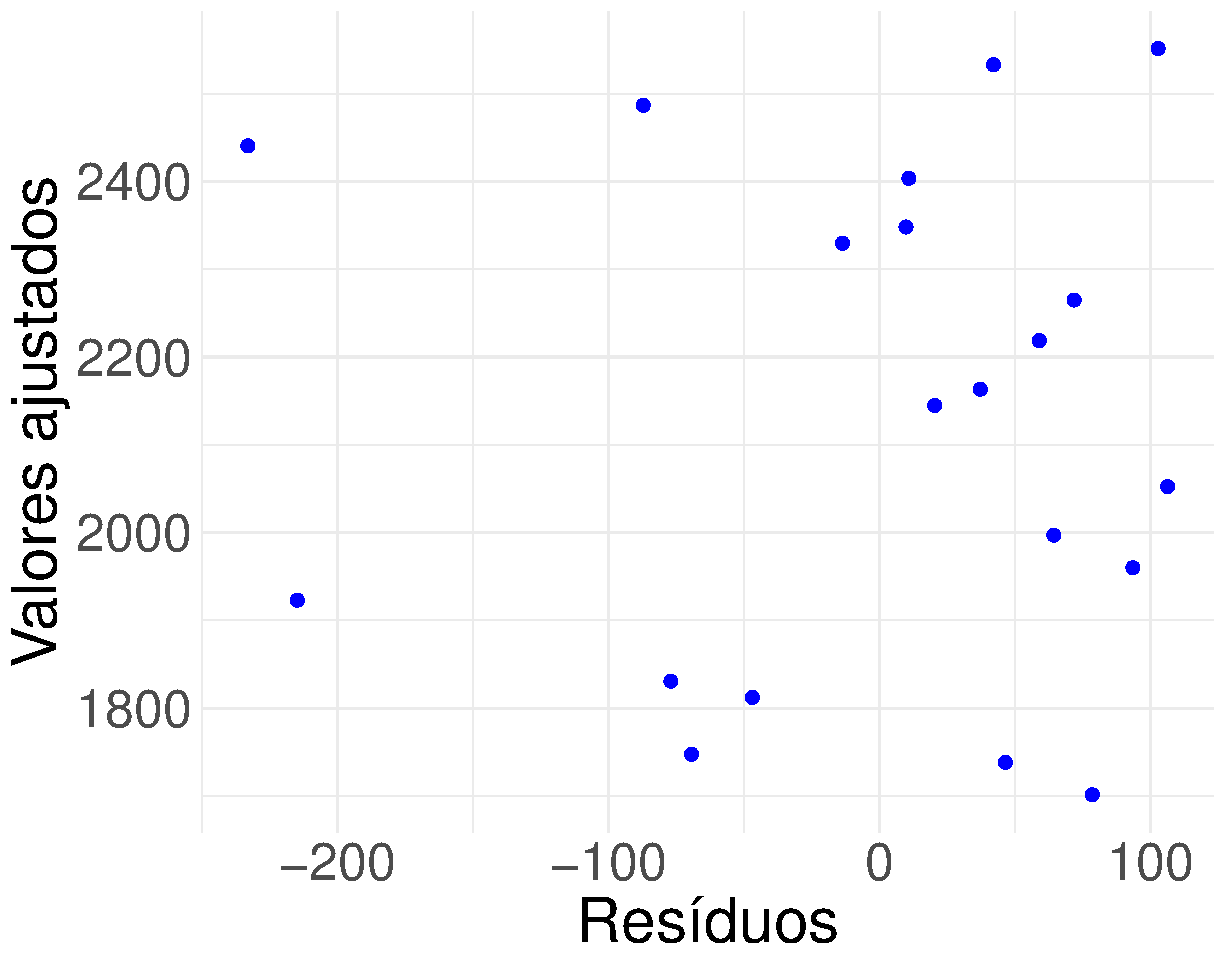
\includegraphics[width=0.25\linewidth]{figure/exemplo-homo.pdf} \label{fig:exemplo-homo}}
		\subfloat[Independência.]{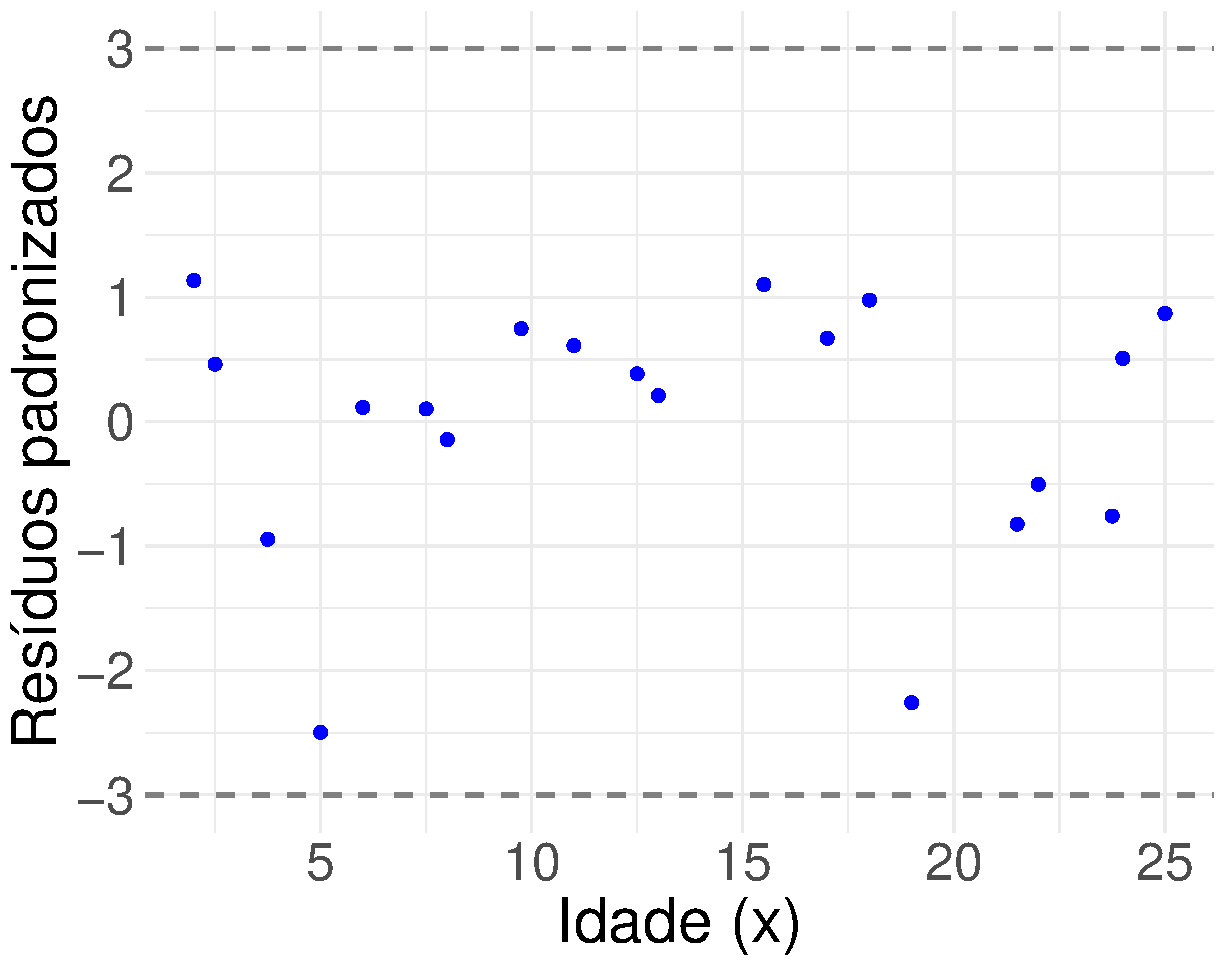
\includegraphics[width=0.25\linewidth]{figure/exemplo-independence-outlier.pdf} \label{fig:exemplo-independence-outlier}}\\
		\subfloat[Linearidade.]{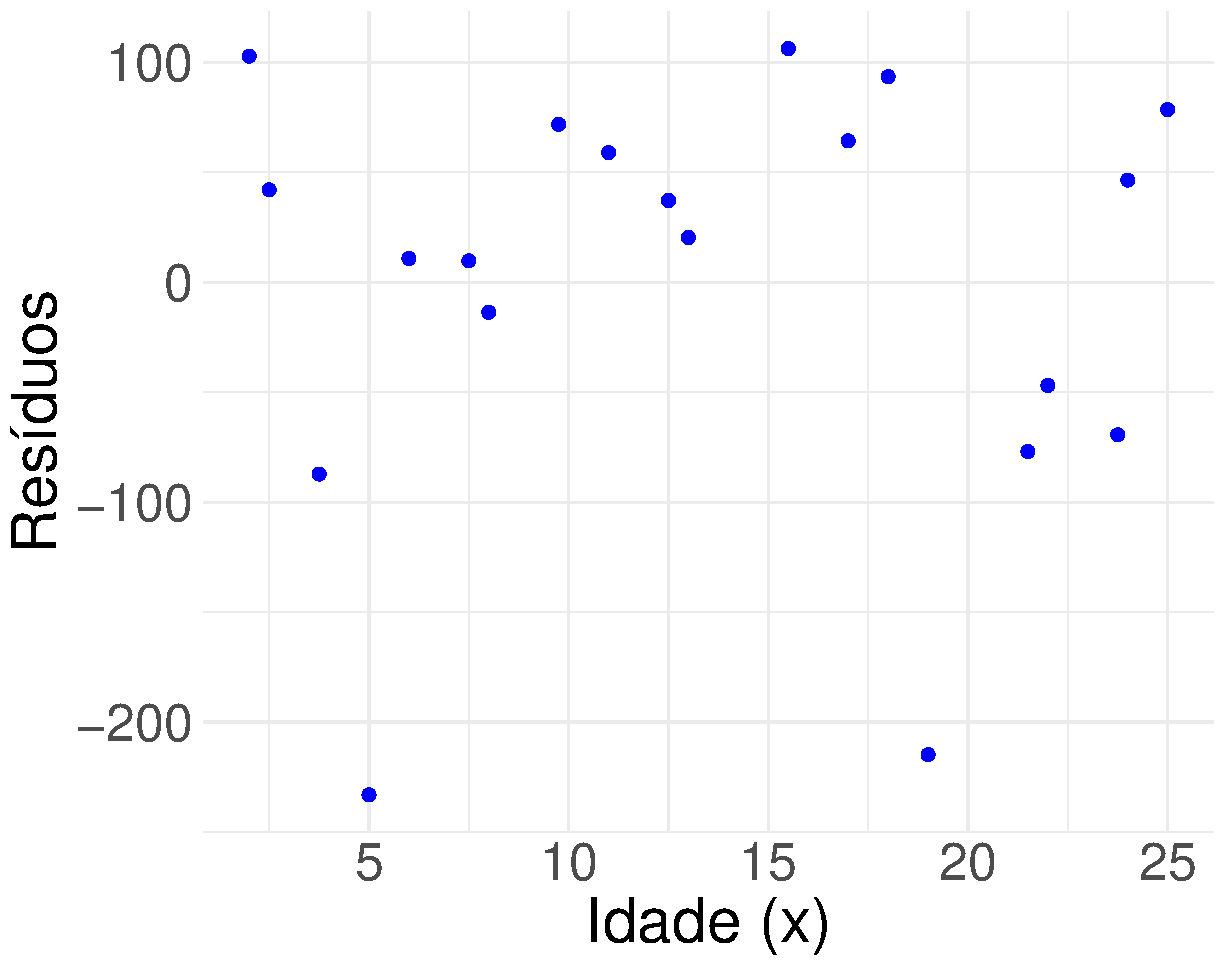
\includegraphics[width=0.25\linewidth]{figure/exemplo-linearity.pdf} \label{fig:exemplo-linearity}}
		\subfloat[Gráfico normal de probabilidade.]{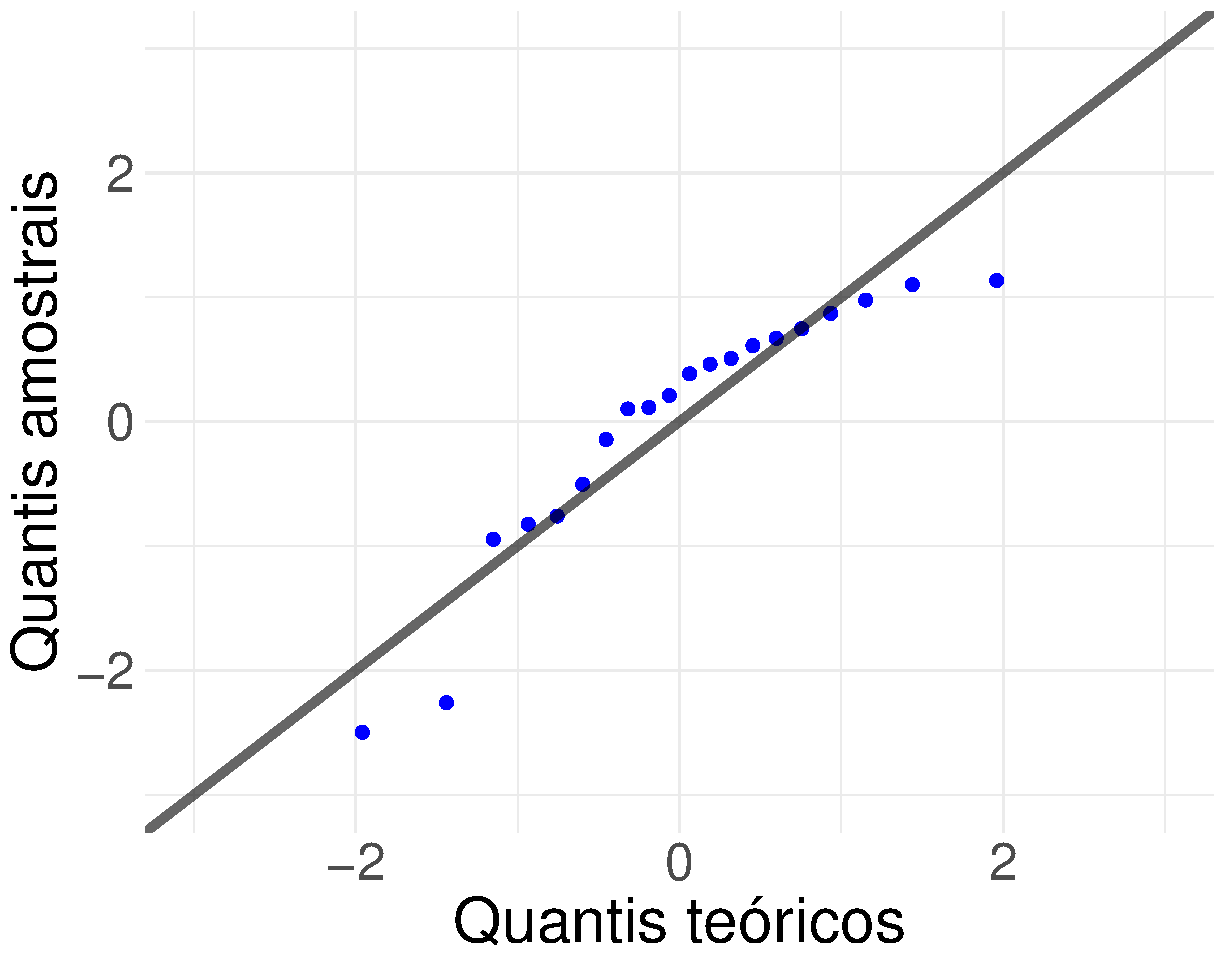
\includegraphics[width=0.25\linewidth]{figure/exemplo-normality.pdf}
		\label{fig:exemplo-normality}}
		\caption{Análise de resíduos.}
	\end{figure}
\end{block}

\end{frame}

\begin{frame}{Exemplo}

\begin{block}{Solução -- análise de resíduos}
	\begin{enumerate}[(a)]
		\item Na Figura~\ref{fig:exemplo-linearity}, não encontramos padrão e tendência. Então, a regressão linear simples, $a + b \cdot x$, é adequada para este conjunto de dados;
		\item Na Figura~\ref{fig:exemplo-independence-outlier}, não encontramos padrão e tendência, e nenhum ponto está abaixo de $-3$ ou acima de $3$. Então, as variáveis aleatórias $\epsilon_i,i=1 \dots, n,$ são independentes e não temos pontos exteriores;
		\item Na Figura~\ref{fig:exemplo-homo}, não encontramos padrão ou tendência. Então, as variáveis aleatórias $\epsilon_i, i=1, \dots, n,$ tem a mesma variância;
		\item Na Figura~\ref{fig:exemplo-normality}, os pontos estão perto da reta $y=x$. Então, as variáveis aleatórias $\epsilon_i, i=1, \dots, n,$ têm distribuição normal.
	\end{enumerate}
\end{block}

\end{frame}

\begin{frame}{Exemplo}

\begin{block}{Solução -- ANOVA.}
	\textbf{Passo 1)} Queremos decidir entre as hipóteses: $H_0;b = 0$ e $H_1;b\neq 0$;
	
	\textbf{Passo 2)} Nível de significância $\alpha=5\%$;
	
	\textbf{Passo 3)} Rejeitamos $H_0$ se $F_0 = \frac{QM_R}{QM_E}$. Ou seja, $RC = \left\{ f_0 \mid f_0 > f_{1-\alpha; 1, n - 2} \right\}$;
	
	\textbf{Passo 4)} Vamos encontrar o valor crítico:
	\begin{itemize}
		\item $P\left( F_{1, n-2} \leq F_{1-\alpha; 1, n-2} \right) = P\left( F_{1, 18} \leq f_{0,95; 1, 18} \right) = 1- \alpha = 0,95$, então $f_{0,95; 1, 18} = 4,4139$;
	\end{itemize}

	\textbf{Passo 5)} Vamos fazer uma Análise de Variância na Tabela~\ref{tab:anova-reg}.
	\begin{table}[ht]
		\centering
		\scalebox{0.65}{
		\begin{tabular}{l|cccc}
			\toprule[0.05cm]
			Fator de variação & Graus de liberdade & Soma dos quadrados & Quadrados médios & $F_0$  \\ 
			\midrule[0.025cm]
			Idade       & 1 & $SQ_R = \hat{b} S_{(x-\bar{x})(y - \bar{y})} =1522819,11$ & $QM_R = \frac{SQ_R}{1} = 1522819,11$ & $\frac{QM_R}{QM_E} = 155,21$  \\ 
			Erro   & 18 & $SQ_E = 176601,82$ & $QM_E = \frac{SQ_E}{n-2} = 9811,21$ &    \\ \midrule[0.025cm]
			Total & 19 & $SQ_T = (n-1)s^2 = 1699420,93$ & & \\
			\bottomrule[0.05cm]
		\end{tabular}
		}
		\caption{Tabela ANOVA para regressão linear simples.} 
		\label{tab:anova-reg}
	\end{table}

	Como $f_0 = 155,21 > f_{0,95;1, 18} = 4,4139$, rejeitamos $H_0$.
\end{block}

\end{frame}

\begin{frame}{Exemplo}
\begin{block}{Solução -- predição para $Y_0 = a + b\cdot x_0 + \epsilon_0$.}
	\begin{itemize}
		\item \textbf{Estimativa pontual} para $Y_0$: $\hat{y}_0 = \hat{a} + \hat{b} x_0 = 2633,28 - 36,84 \cdot 20 = 1896,48$;
		
		\item \textbf{Intervalo de confiança} para $Y_0$. Primeiro calculamos os quantis:
		\begin{itemize}
			\item $P(t_{n-2} = t_{\frac{\alpha}{2};n-2}) = P(t_{18} = t_{0,025;18}) = \frac{\alpha}{2} = 0,025$, então $t_{0,025;18} = -2,101$;
			\item $P(t_{n-2} = t_{\frac{\alpha}{2};n-2}) = P(t_{18} = t_{0,975;18}) = 1-\frac{\alpha}{2} = 0,975$, então $t_{0,975;18} =  2,101$;
		\end{itemize}
		Note que $\hat{\sigma} = 9811,21$, $x_0 = 20$,  $\bar{x} = 13,34$ e $S_{(x-\bar{x})} = 1114,659$. Então o intervalo de confiança com coeficiente de confiança $\gamma = 95\%$ é dado por:
		\small
		\begin{align*}
			IC(Y_0, \gamma) &= \left( t_{\frac{\alpha}{2}; n-2} \sqrt{\hat{\sigma}^2 \left[ 1 + \frac{1}{n} + \frac{(x_0 - \bar{x})^2}{S_{(x - \bar{x})^2}} \right]} + \hat{y}_0; t_{1-\frac{\alpha}{2}; n-2} \sqrt{\hat{\sigma}^2 \left[ 1 + \frac{1}{n} + \frac{(x_0 - \bar{x})^2}{S_{(x - \bar{x})^2}} \right]} + \hat{y}_0 \right)\\
			&= \left(-2,101 \cdot \sqrt{9811,212 \left[ 1 + \frac{1}{20} + \frac{(20 - 13,24)^2}{1114,659}  \right]} + 1896,48;\right.\\
			&\qquad\qquad \left. 2,101 \cdot \sqrt{9811,212 \left[ 1 + \frac{1}{20} + \frac{(20 - 13,24)^2}{1114,659}  \right]} + 1896,48 \right) \\
			&= \left( 1679,23; 2113,73  \right)
		\end{align*} 
		\normalsize
	\end{itemize}	

	A força da liga para um proponente com 20 semanas está entre $1679,23$ e $2113,73$ com coeficiente de confiança $\gamma=95\%$.
\end{block}
\end{frame}

\end{document}


